% SigDrop journal draft v1 (2026-11-16). Build: ./build.sh  -> main.pdf
% Every number is traced in ../README-vi.md (measured in ns-3 / computed from logs / carried over from the ICC draft).
\documentclass[journal,10pt]{IEEEtran}
\usepackage[T1]{fontenc}
\usepackage[utf8]{inputenc}
\usepackage{amsmath,amssymb,amsthm}
\usepackage{graphicx}
\usepackage{booktabs}
\usepackage{algorithm}
\usepackage{algorithmic}
\usepackage{cite}
\usepackage{xcolor}
\usepackage{url}
\graphicspath{{../figs/}}
\newtheorem{theorem}{Theorem}
\newtheorem{proposition}{Proposition}
\newtheorem{corollary}{Corollary}
\newtheorem{lemma}{Lemma}
\theoremstyle{definition}
\newtheorem{definition}{Definition}
\theoremstyle{remark}
\newtheorem{remark}{Remark}
\newcommand{\todo}[1]{\textcolor{red}{[TODO: #1]}}
\newcommand{\Tp}{T_{\mathrm p}}
\newcommand{\spine}{\textsc{Spine}}
\newcommand{\lmtour}{\textsc{LM-Tour}}
\newcommand{\chord}{\textsc{Chord}}
\DeclareMathOperator*{\argmin}{arg\,min}
\renewcommand{\algorithmicrequire}{\textbf{Input:}}

\begin{document}
\title{Flight Geometry Is the Schedule: Pre-Planned Ground Cooperation for Single-Pass UAV Query Delivery to Edge-Camera Networks}
\author{\todo{authors and affiliations}%
\thanks{Draft v1 of the journal version (2026-11-16). A preliminary version was submitted to IEEE ICC 2027.}}
\maketitle

\begin{abstract}
To find a missing person quickly, a search query---a set of reference images of several hundred kilobytes---must reach
the few AI-capable cameras of a large IoT network that has no broadband backhaul. A fixed-wing UAV can broadcast the
query over IEEE 802.15.4, but it crosses each cluster once, and its air-to-ground range varies from about 1\,km over open
land to below 100\,m under canopy. We observe that in a single-pass broadcast the flight geometry \emph{is} the
transmission schedule: before take-off the base station knows which segment of the packet stream is emitted above which
cell, and can plan both the path and the ground cooperation. This paper develops that idea into a complete system and a
theory of when it pays off. We formulate joint trajectory and ground-transport design and show it is NP-hard. We prove a
lower bound on the completion time of \emph{every} scheme in which cameras rely only on what their own cell hears from the
UAV, whatever its trajectory and code: the time is at least the query airtime multiplied by a fractional covering number
$\Lambda^\star$ of the cameras, computed by a linear programme, whereas a single pass needs the query airtime once per
cluster. On our maps $\Lambda^\star$ grows from 4--7 over open land to 35--76 at 100\,m range. On the system side,
\textsc{River} is a pre-planned cell-level transport (\spine{} $\to$ Bank $\to$ Ring $\to$ critical cell) with a
\emph{takeover} repair that keeps the plan valid under trajectory error, and \lmtour{} designs the flight for the ground
transport using a surrogate learned from ns-3. In ns-3 with a full 802.15.4 MAC, on maps of 8--15 clusters,
\lmtour{}+\textsc{River} shortens the mission by 59--72\,\% against fountain-coded loitering when the range is 200\,m or
less, finishes its whole flight before the proven limit of non-cooperative delivery, needs 1.9--2.5$\times$ fewer frames
than Deluge, and under 100\,m cross-track error the takeover completes every camera with unchanged mean mission time.
\end{abstract}
\begin{IEEEkeywords}
UAV, single-pass broadcast, IEEE 802.15.4, cooperative dissemination, Dubins traveling salesman problem, lower bounds,
edge AI, search and rescue.
\end{IEEEkeywords}

\section{Introduction}
UAVs inspect power lines, map crops, deliver medicine and extend cellular coverage after disasters
\cite{zeng2016mag,mozaffari2019}. Most of these uses make an existing service faster or cheaper. UAVs also enable
operations that did not exist before because no infrastructure could support them: urgent, one-off missions in places
where the network is weak.

Searching for a missing person is such a mission. A lost hiker or a missing child has often walked past many cameras
installed by different owners at different times. A few of them, or an edge box attached to them, can run a neural
matcher; most are legacy devices that only record. None knows whom to look for. Where an AI camera has broadband, the
query can simply be sent to it; our concern is the large remainder in mountain resorts, parks and along rural roads, where
devices are linked only by low-power radios and footage cannot be uploaded. We therefore push a compact query down
instead of pulling footage up. In a network built by many owners the AI nodes run different embedding models whose
vectors are not comparable \cite{shen2020}; the query must carry reference images so that each node embeds them with its
own model. We use $L=12$ images, about 400\,kB, i.e., $Q=4041$ packets, as the nominal case.

\textbf{Challenge.} A fixed-wing UAV covers a large area but cannot hover; it crosses each cluster once. One copy of the
query takes about 2\,km of flight. If the air-to-ground (A2G) range is about 1\,km (open land), nodes far from the path
still receive many packets, but scattered, so few complete an image. If the range is 100--200\,m (canopy, tall buildings),
a cell hears only the few hundred packets emitted while the UAV is overhead. Either way the AI nodes, which are rarely on
the path, cannot assemble the query alone. The classical answers are to make the UAV dwell near every receiver until it
has decoded a rateless code \cite{zeng2018multicast,luby2002}, or to let the ground disseminate the object epidemically
\cite{hui2004,levis2004}. The first costs airtime at every receiver; the second discovers at run time what the base
station (BS) could have known in advance.

\textbf{Key insight.} Packet $s$ is emitted at a point $\gamma(d_0+s\Delta)$ of a path $\gamma$ that the BS designs.
Before take-off the BS therefore knows which segment of the stream lands on which cell, and can plan both the path and the
ground cooperation: \emph{the flight geometry is the transmission schedule}.

\textbf{Contributions.} This paper extends our conference version \todo{cite ICC 2027 submission} with a formal problem
statement, fundamental limits, a repair mechanism for trajectory errors and a substantially larger evaluation.
\begin{enumerate}
\item \emph{Formulation and complexity.} We state single-pass query delivery as a joint choice of a curvature-constrained
trajectory and a ground forwarding schedule, and prove that it is NP-hard already without ground links
(Section~\ref{sec:problem}).
\item \emph{Limits of non-cooperative delivery.} For every scheme in which a camera uses only what its own cell hears,
we prove that the completion time is at least $(1-\delta)\,Q\,\Tp\,\Lambda^\star$, where $\Lambda^\star$ is a fractional
covering number of the critical cells under the reception footprint, obtained from a linear programme. The bound holds
for any trajectory, any code and correlated fading, and yields a sufficient condition under which ground cooperation
is strictly faster, including the case of no-fly zones (Section~\ref{sec:limits}).
\item \emph{River.} A pre-planned, cell-level transport, \spine{}\,$\to$\,Bank\,$\to$\,Ring\,$\to$\,critical cell, that
needs no route or content discovery, together with \emph{takeover}, a repair that restores delivery when the real
trajectory deviates from the plan, a characterisation of when it is triggered, and a single-radio lower bound against
which we measure River's ground time (Section~\ref{sec:river}).
\item \emph{Flight design.} \chord{} and \lmtour{}, which choose the path for the ground transport rather than for
coverage, the latter guided by a surrogate of River's completion time learned from ns-3 (Section~\ref{sec:flight}).
\item \emph{Evaluation} in ns-3 with a full 802.15.4 MAC over three maps, four A2G regimes and up to ten network
realisations per setting: mission time, the measured schemes against the proven limits, frames and radio energy
against Deluge and planned direct pulling, and robustness to trajectory error (Section~\ref{sec:eval}).
\end{enumerate}

\section{Related Work}\label{sec:related}
\textbf{UAV-enabled multicasting.} UAV trajectories are routinely optimised jointly with communication
\cite{zeng2016mag,mozaffari2019,wu2018,zeng2017energy}. Closest to our baseline, Zeng \emph{et al.}
\cite{zeng2018multicast} minimise the time for every ground terminal to recover a common file, coded with random linear
network coding, directly from a rotary-wing UAV. They lower-bound the recovery probability by the time the UAV spends
within a distance $D$ of each terminal, which turns the design into a waypoint problem, and they name a subsequent
device-to-device sharing phase as future work. Sharing among users after an aerial multicast has since been studied for
one-hop D2D links in cellular settings \cite{wang2020d2d,miao2020}. We consider the opposite end of the design space: a
fixed-wing UAV that cannot dwell, receivers that are a known subset of a multi-hop 802.15.4 mesh, and cooperation that is
planned from the trajectory before take-off. Our lower bound (Theorem~\ref{thm:cover}) applies to the whole class of
direct-reception designs, including \cite{zeng2018multicast}.

\textbf{Bulk dissemination in sensor networks.} Deluge \cite{hui2004} and Trickle \cite{levis2004} spread an object to
every node by advertise--request epidemics. MNP lets nodes sleep while neighbours send segments they do not need
\cite{kulkarni2005}; Typhoon uses unicast with snooping and channel switching \cite{liang2008}; Splash and Pando build on
constructive interference and reach an order of magnitude lower dissemination time than Deluge on testbeds
\cite{doddavenkatappa2013,du2017}; the Low-Power Wireless Bus schedules all communication centrally over synchronous
floods \cite{ferrari2012}. All of them start from a sink and target every node. River differs in where the data enters
(a known segment at every cell under the path), in whom it targets (a few critical cells) and in that the complete
forwarding plan follows from the flight geometry. Fountain and network codes \cite{luby2002,shokrollahi2006,ho2006}
relax \emph{which} packets are needed but not \emph{where} they are; River is compatible with both. For a single
broadcast channel, Stojanovic \emph{et al.} \cite{stojanovic2009} compare coded retransmission with cooperation among
receivers and find a crossover in the erasure probability; our crossover is geometric and involves the trajectory.

\textbf{Curvature-constrained routing.} The Dubins traveling salesman problem (DTSP) is NP-hard \cite{leny2012}; with
neighbourhoods (DTSPN) it is solved in practice by sampling entry configurations and transforming the resulting
generalised TSP into an asymmetric TSP \cite{isaacs2011,noon1993,obermeyer2009}, and data-collection variants add travel
budgets \cite{penicka2019}. Our tours use these building blocks, but the objective is the readiness time of the ground
transport rather than tour length.

\textbf{A2G channels and flight accuracy.} Low-altitude A2G propagation depends strongly on environment and elevation
angle \cite{khawaja2019,alhourani2014,matolak2017}, and field measurements of 2.4\,GHz 802.15.4 links from UAVs report
ranges well below nominal \cite{nekrasov2019}. We therefore treat the range as a regime parameter. Small fixed-wing
aircraft follow planned paths within metres under moderate wind \cite{park2007,nelson2007}; turns planned in still air
are distorted by wind \cite{techy2009}, which motivates the repair of Section~\ref{sec:takeover}.

\textbf{Person search at the edge.} Face recognition and person re-identification compare a probe with stored crops by
cosine similarity of learned embeddings \cite{schroff2015,deng2019,ye2022}; embeddings of different models are
incompatible \cite{shen2020}. We use these results only to define the query and the value of partial data.

\section{System Model}\label{sec:model}
\subsection{Network and organisation}
The area is tiled by hexagonal cells of radius $R_{\mathrm c}=100$\,m. The static nodes form an IEEE 802.15.4 mesh that
is organised once, before any mission (\emph{phase~0}): every cell has a cell leader (CL); two adjacent cells are joined
by exactly one gateway pair; cell channels follow a 7-colour reuse and every gateway pair has its own radio and channel;
cell-level routes are precomputed. Cells are grouped into clusters of at most 80 cells, each with a cluster head (CH) that
has a LoRa uplink to the BS. Let $G=(V,E)$ be the graph whose vertices are cells and whose edges are gateway pairs. A
subset $K\subseteq V$ of \emph{critical cells} hosts an AI node (a smart camera or an edge box); the other cameras are
legacy devices that detect motion and keep event crops in a ring buffer.

\subsection{UAVs and emission}
Team~1 is a fixed-wing UAV at altitude $h=100$\,m with speed $v\in[25,50]$\,m/s and bank angle at most $45^\circ$, hence a
turning radius $\rho(v)=v^2/g$: 255\,m at 50\,m/s and 63.7\,m at 25\,m/s. It broadcasts one packet of $B=99$\,B payload
every $\Tp=10$\,ms, i.e., every $\Delta=v\Tp\le 0.5$\,m. Its ground track is a curve $\gamma$ from and to the BS; packet
$s$ is emitted at $x_s=\gamma(s\Tp)$. Team~2 is a rotary-wing UAV (15\,m/s) that verifies candidate cells in phase~2.

\subsection{Air-to-ground reception}
At slant distance $\ell=\sqrt{d^2+h^2}$ the path loss is free space up to $d_0=100$\,m ($PL_0=80.05$\,dB at 2.4\,GHz)
and grows with exponent $\alpha=3$ beyond, plus an excess loss $L_{\mathrm{obs}}$ of the environment:
\begin{equation}
PL(\ell)=PL_0+10\alpha\log_{10}(\ell/d_0)+L_{\mathrm{obs}},\qquad \ell\ge d_0 .\label{eq:pl}
\end{equation}
Each packet sees independent Rician fading with $K=2$ (Nakagami $m=1.8$ in ns-3) and is received when the faded power
exceeds an effective threshold $S$. With $P_{\mathrm t}=10$\,dBm, a node at horizontal distance $d$ receives a packet with
probability
\begin{equation}
p(d)=\Pr\bigl\{g>10^{(S-P_{\mathrm t}+PL(\ell))/10}\bigr\},\quad 2(K{+}1)g\sim\chi'^2_2(2K).\label{eq:pd}
\end{equation}
We summarise a regime by $R_{50}$, the horizontal distance at which $p=1/2$. The four regimes of this paper,
$L_{\mathrm{obs}}=0$, 9.0, 19.8 and 25.7\,dB, give $R_{50}=1016$, 498, 199 and 99\,m. A single threshold
$S=-101.04$\,dBm (nominal sensitivity $-100$\,dBm) reproduces the reception measured on the ns-3 passes in all four
regimes with a root-mean-square error of at most 0.003 (Fig.~\ref{fig:channel}).

The CL gathers what the nodes of its cell hold, so the relevant event is that \emph{some} node of the cell hears the
packet. For a cell $k$ with node set $U_k$ and a UAV at horizontal position $x$,
\begin{equation}
P_k(x)=1-\prod_{u\in U_k}\bigl(1-p(\lVert x-u\rVert)\bigr).\label{eq:pcell}
\end{equation}
Equation~\eqref{eq:pcell} assumes independent receptions across nodes (A1). The limits of Section~\ref{sec:limits} need
only the marginal probabilities $P_k(x)$ and no independence across packets.

\begin{figure}[t]\centering
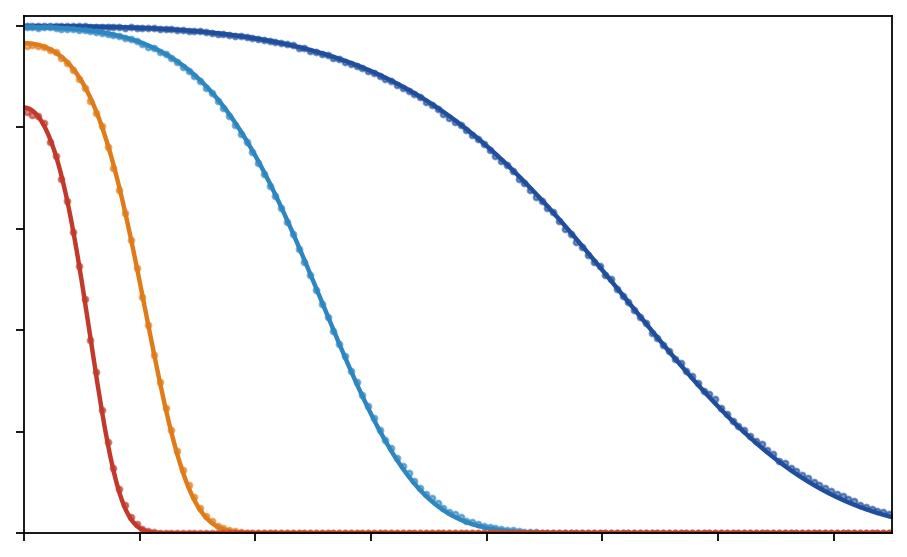
\includegraphics[width=0.86\columnwidth]{nd1-channel-p-of-d-model-vs-ns3.png}
\caption{Packet reception versus horizontal distance (0 to 1.5\,km; vertical axis 0 to 1) for the four regimes, from
$R_{50}=1016$\,m (rightmost) to 99\,m. Dots: measured on ns-3 passes in 10\,m bins. Lines: model \eqref{eq:pd} with one
common threshold. \todo{labelled version of this plot}}\label{fig:channel}
\end{figure}

\subsection{Ground medium}
Ground links follow exponent 3.5 with log-normal shadowing ($\sigma=7.8$\,dB, drawn once per node pair) and Rayleigh
fading in 100\,ms blocks \cite{tr38901}. Every cell and every gateway pair is one \emph{medium}: at most one of its
radios transmits at a time, under CSMA/CA with acknowledgements and retransmissions. An acknowledged hop of a 127\,B frame
occupies its medium for at least $\tau_{\min}=4.8$\,ms (4.256\,ms frame, turnaround, ACK) and for $\tau_f\approx5$--7\,ms
in practice.

\subsection{Query, coding and completion}
The query consists of $L=12$ reference images, $Q=4041$ packets in total. Each image is atomic. The UAV repeats the
query along its path; with a rateless code a cell decodes once it holds $N'=\lceil(1+\epsilon)Q\rceil$ distinct coded
packets ($\epsilon=0.05$), and no code can decode from fewer than $Q$ packets. The \emph{completion time} $C_k$ of
critical cell $k$ is the first time at which its CL holds enough packets to decode the query.

\subsection{Mission time}
After completion, the AI node matches the query against its stored crops and reports one flag and a 2-byte bitmap
through its CH over LoRa (one message per 40\,s under the duty cycle \cite{etsi220}); the BS updates the posterior of each
cell and Team~2 visits cells in decreasing order of posterior per unit time, each verification taking about 78\,s. The
mission time $T^\star$ is the time at which a cell that truly saw the target is verified. The matching layer is the one
of the conference version; it is common to all schemes, and all schemes are compared on the same draws.

\section{Problem Formulation and Complexity}\label{sec:problem}
\subsection{Joint design problem}
A \emph{plan} consists of (i) a trajectory: a ground track $\gamma:[0,T_{\mathrm f}]\to\mathbb{R}^2$ with
$\gamma(0)=\gamma(T_{\mathrm f})$ at the BS, speed in $[v_{\min},v_{\max}]$ and curvature at most $1/\rho(v)$, possibly
restricted to a set $F$ of allowed positions (no-fly zones); and (ii) a ground schedule $\pi$: a causal rule that, at any
time, selects for every medium at most one transmitter and one packet that this transmitter holds, each transmission
occupying the medium for $\tau_f$. Receptions from the UAV are random according to \eqref{eq:pd}. The joint problem is
\begin{equation}
\begin{aligned}
\textbf{(P0)}\quad &\min_{\gamma,\pi}\ \mathbb{E}\bigl[\Phi(C_1,\dots,C_{|K|})\bigr]\\
&\ \text{s.t.}\ \Pr\bigl\{\max\nolimits_k C_k\le T_{\max}\bigr\}\ge 1-\delta ,
\end{aligned}\label{eq:p0}
\end{equation}
where $\Phi$ is the makespan $\max_k C_k$ or a weighted sum $\sum_k w_kC_k$. The makespan is the natural measure of the
delivery layer; the weighted sum is what the mission time $T^\star$ responds to, since every completed cell lets the BS
refine its posterior.

(P0) couples a continuous curvature-constrained routing problem with a multi-commodity scheduling problem through the
\emph{reception map}: the trajectory decides which cell holds which packets. We decompose it. For a fixed trajectory,
the BS predicts the reception map from \eqref{eq:pcell} and plans the ground transport (River, Section~\ref{sec:river});
the flight planner then searches over trajectories using a fast predictor of the ground completion times
(Section~\ref{sec:flight}).

\subsection{Complexity}
\begin{theorem}\label{thm:nphard}
The decision version of (P0) with the makespan objective---given $T$, is there a plan under which every critical cell is
complete and the UAV is back at the BS by time $T$---is NP-hard. It remains NP-hard for a single UAV of constant speed,
deterministic reception and a ground graph without edges.
\end{theorem}
The proof (Appendix~\ref{app:nphard}) follows Le Ny \emph{et al.}'s reduction for the DTSP \cite{leny2012}: an instance
of Exact Cover is mapped, through Papadimitriou's construction for the Euclidean TSP \cite{papadimitriou1977} and a
rescaling that absorbs both the turning-radius penalty of Savla \emph{et al.} \cite{savla2008} and the reception radius,
to an instance in which every critical cell must be overflown. The theorem locates the hardness in the flight layer and
justifies the heuristics of Section~\ref{sec:flight}; it says nothing about the ground schedule for a fixed trajectory,
for which Section~\ref{sec:river} gives a lower bound.

\section{Limits of Non-Cooperative Delivery}\label{sec:limits}
Before designing cooperation we ask what any design without it can achieve.

\begin{definition}
A delivery scheme is \emph{non-cooperative} if every critical cell decodes only from packets that nodes of its own cell
received from the UAV. The trajectory, the speed profile, the code and the in-cell gathering are arbitrary.
\end{definition}
The class contains loitering with a rateless code \cite{zeng2018multicast}, both fountain-coded baselines of
Section~\ref{sec:eval}, and a hovering rotary-wing transmitter.

\subsection{A covering bound}
Let $F\subseteq\mathbb{R}^2$ be the set of horizontal positions the UAV may occupy and $P_k(x)$ the cell-level reception
probability \eqref{eq:pcell}. Consider the linear programme
\begin{equation}
\Lambda^\star=\max_{\lambda\ge0}\ \sum_{k\in K}\lambda_k\quad\text{s.t.}\quad \sum_{k\in K}\lambda_kP_k(x)\le1\ \ \forall x\in F.
\label{eq:lp}
\end{equation}
\begin{theorem}[Covering bound]\label{thm:cover}
Consider a non-cooperative scheme whose trajectory is fixed before take-off. If every critical cell is complete by time
$T$ with probability at least $1-\delta$, then
\begin{equation}
T\ \ge\ (1-\delta)\,Q\,\Tp\,\Lambda^\star .\label{eq:cover}
\end{equation}
\end{theorem}
\begin{IEEEproof}
Let $x_1,\dots,x_n$ be the emission positions up to time $T$, $n\le T/\Tp$, and $N_k$ the number of these packets heard
by at least one node of cell $k$. No code recovers $Q$ packets of information from fewer than $Q$ received packets, so
completion requires $N_k\ge Q$ and $\mathbb{E}[N_k]\ge Q\Pr\{N_k\ge Q\}\ge(1-\delta)Q$. By linearity of expectation
$\mathbb{E}[N_k]=\sum_{s=1}^nP_k(x_s)$. For any $\lambda$ feasible in \eqref{eq:lp},
\[
(1-\delta)Q\sum_k\lambda_k\le\sum_k\lambda_k\!\sum_{s=1}^n\!P_k(x_s)=\sum_{s=1}^n\sum_k\lambda_kP_k(x_s)\le n .
\]
Maximising over $\lambda$ gives $n\ge(1-\delta)Q\Lambda^\star$ and $T\ge n\Tp$.
\end{IEEEproof}

\begin{remark}[What $\Lambda^\star$ measures]
With $\bar p_k=\sup_{x\in F}P_k(x)$ we have $\max_k1/\bar p_k\le\Lambda^\star\le\sum_k1/\bar p_k$. If one position serves
every critical cell with probability one, $\Lambda^\star=1$: one airtime of the query suffices. If the reception
footprints are disjoint, $\Lambda^\star=\sum_k1/\bar p_k\ge|K|$: every critical cell needs its own airtime. In between,
$\Lambda^\star$ is the fractional number of critical cells that cannot be served simultaneously. By LP duality,
$\Lambda^\star$ is also the smallest total dwell, in units of $Q\Tp$, of a transmitter that could hover anywhere in $F$
and serve every cell in expectation; the bound is therefore tight, up to travel time and a concentration margin, for a
rotary-wing transmitter, and it can only be looser for a fixed-wing one.
\end{remark}
\begin{remark}[Robustness]
The proof uses only marginal reception probabilities. It holds for any dependence of fading across packets, for any code
and for any number of passes. Independence across the nodes of one cell enters only through the product form
\eqref{eq:pcell} of $P_k$.
\end{remark}

\subsection{Adding travel}
The covering bound ignores that the UAV must move between receivers. A second bound accounts for it when receivers are
far apart. For a radius $D$ let $p_k(D)=\sup\{P_k(x):\lVert x-c_k\rVert\ge D\}$, with $c_k$ the centre of cell $k$.
\begin{proposition}[Packing bound with travel]\label{prop:pack}
Let $S\subseteq K$ be critical cells whose centres are pairwise more than $2D$ apart, and let $W(S)$ be the weight of a
minimum spanning tree of $\{c_k\}_{k\in S}$ and the BS. Under the assumptions of Theorem~\ref{thm:cover},
\begin{equation}
\begin{aligned}
T\ \ge\ \min\Biggl\{&\frac{b\sum_{k\in S}\bar p_k^{-1}+(W(S)-2D|S|)^+/v_{\max}}{1+\sum_{k\in S}p_k(D)/\bar p_k},\\
&\frac{b}{\max_{k\in S}p_k(D)}\Biggr\},\qquad b=(1-\delta)Q\Tp .
\end{aligned}\label{eq:pack}
\end{equation}
\end{proposition}
The proof is in Appendix~\ref{app:pack}: emissions inside the disc of radius $D$ around $c_k$ serve $k$ with probability
at most $\bar p_k$, all others with at most $p_k(D)$; the discs are disjoint, and the path outside them connects them.
The second term of the minimum is the time before which no cell of $S$ can be served from outside its disc; it is not
binding in our evaluations.

\subsection{When cooperation is faster}
A single-pass scheme with ground cooperation must offer every cluster one copy of the query on its own cells, so its
flight lasts $T_{\mathrm{fly}}=\sum_c\max(\ell_c/v_c,\,Q\Tp)+T_{\mathrm{transit}}$, where $\ell_c$ is the path length
inside cluster $c$; the ground then needs a time $T_{\mathrm g}$ after the UAV has left.
\begin{corollary}[Sufficient condition]\label{cor:cross}
If a cooperative scheme completes every critical cell by
$T_{\mathrm{coop}}<(1-\delta)Q\Tp\Lambda^\star$, it completes before every non-cooperative scheme, whatever the latter's
trajectory and code.
\end{corollary}
Cooperation thus pays the query airtime $Q\Tp$ once per \emph{cluster}, while non-cooperation pays it once per unit of
$\Lambda^\star$. As the A2G range shrinks, $\Lambda^\star$ grows towards $|K|$ and beyond, whereas the number of clusters
is fixed by the network organisation.

\begin{corollary}[No-fly zones]\label{cor:nofly}
If $F$ excludes a region such that $\sup_{x\in F}P_k(x)=0$ for some critical cell $k$, then $\Lambda^\star=\infty$: no
non-cooperative scheme completes. A cooperative scheme is unaffected as long as the cell graph connects $k$ to cells
under the allowed path.
\end{corollary}

\subsection{Numerical evaluation}
We solve \eqref{eq:lp} on the three maps of Section~\ref{sec:eval} with the positions $x$ on a 50\,m grid and rescale
$\lambda$ by the maximum of $\sum_k\lambda_kP_k(x)$ on a 20\,m grid, so that the reported value is feasible on the finer
grid; \eqref{eq:pack} is maximised over $D$ and greedy choices of $S$. We take $\delta=0.1$ and $v_{\max}=50$\,m/s.
Table~\ref{tab:bounds} and Fig.~\ref{fig:bounds} compare the bounds with the measured schemes.

\begin{table}[t]\centering
\caption{Fractional covering number $\Lambda^\star$ and lower bounds on any non-cooperative scheme (s), against the
measured flight end of the fountain-coded baseline and of the single-pass flights (s). Maps with 8 / 12 / 15 clusters
and 45 / 66 / 92 critical cells.}\label{tab:bounds}
\setlength{\tabcolsep}{3pt}\footnotesize
\begin{tabular}{llrrrrrr}\toprule
Map & $R_{50}$ & $\Lambda^\star$ & \eqref{eq:cover} & \eqref{eq:pack} & FC+DTSP-N & \chord & \lmtour\\\midrule
8  & 1016 & 4.0  & 146  & 123  & 669  & 784  & 698\\
   & 498  & 10.0 & 362  & 256  & 1320 & 784  & 699\\
   & 199  & 23.2 & 842  & 610  & 2687 & 784  & 697\\
   & 99   & 35.3 & 1283 & 880  & 3305 & 784  & 708\\\midrule
12 & 1016 & 5.5  & 201  & 157  & 913  & 1292 & 1085\\
   & 498  & 14.1 & 511  & 339  & 2011 & 1292 & 1085\\
   & 199  & 33.5 & 1220 & 865  & 4016 & 1292 & 1083\\
   & 99   & 53.6 & 1951 & 1375 & 5078 & 1292 & 1082\\\midrule
15 & 1016 & 7.0  & 254  & 163  & 1134 & 1437 & 1394\\
   & 498  & 18.0 & 655  & 400  & 2563 & 1437 & 1308\\
   & 199  & 47.1 & 1713 & 1051 & 5567 & 1437 & 1293\\
   & 99   & 76.4 & 2779 & 1731 & 6808 & 1437 & 1291\\\bottomrule
\end{tabular}
\end{table}

\begin{figure*}[t]\centering
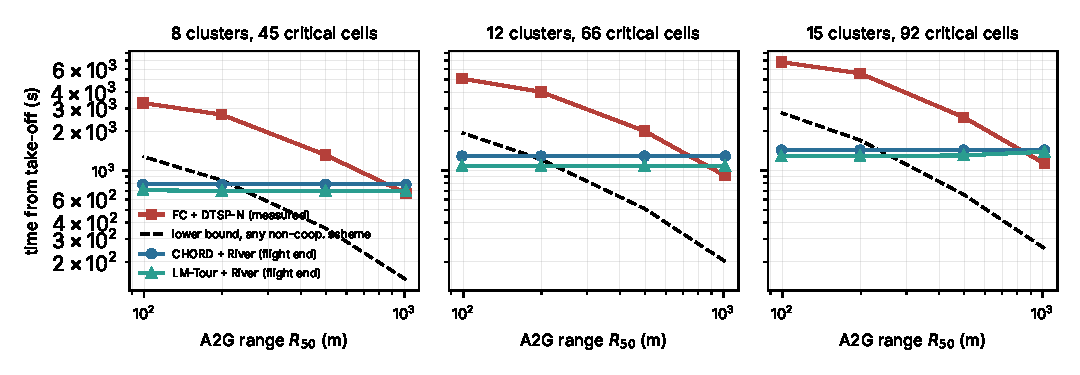
\includegraphics[width=0.86\textwidth]{bound-lp.pdf}
\caption{Lower bound on any non-cooperative scheme (maximum of \eqref{eq:cover} and \eqref{eq:pack}, dashed) against
the measured flight end of FC+DTSP-N and of the two single-pass flights, versus A2G range.}\label{fig:bounds}
\end{figure*}

Three observations follow. First, $\Lambda^\star$ grows by an order of magnitude from open land to $R_{50}=99$\,m, from
4--7 to 35--76, i.e., from below the number of clusters to several times it. Second, for $R_{50}\le200$\,m the covering
bound exceeds the time at which \lmtour{} has finished its \emph{entire} flight, return leg included, on all three maps
(e.g., 1713\,s against 1293\,s on the largest map at 199\,m), and at 99\,m it exceeds \chord's flight as well. On the
8-cluster map at 99\,m, where we have per-cell completion times, the last critical cell completes 746\,s after take-off
with \chord{}+River, against a bound of 1283\,s: no non-cooperative design, however it flies and codes, can match the
single pass there. Third, the bound is 2.4--4.6 times below the measured fountain-coded baseline. The gap has three
sources: the bound allows the transmitter to hover at the best position, it uses an ideal code without margin, and the
baseline's orbit and visiting order are heuristic. At $R_{50}\ge500$\,m the bound lies below the single-pass flight time
and certifies nothing, although the measured baseline is still slower from 500\,m downwards (Section~\ref{sec:eval}).

\emph{No-fly zone.} On the 8-cluster map we forbid the UAV to fly within a radius $\varrho$ of the centre of the cluster
with most critical cells. For $\varrho=400$\,m (two critical cells inside) the bound is unchanged. For $\varrho=700$\,m
(four inside) it stays at 145--363\,s for $R_{50}\ge498$\,m, jumps from 842 to 3431\,s at 199\,m, and is infinite at
99\,m: the cells deep inside cannot be reached from the air at all. \todo{ns-3 run of River with a path that avoids the
zone; not yet simulated.}

\section{River: Pre-Planned Ground Transport}\label{sec:river}
\subsection{Roles and plan}
For a path $\gamma$ through a cluster, the \spine{} is the ordered list of cells that $\gamma$ crosses, and
$\mathrm{Seg}(a)=\{s:\gamma(s\Tp)\in a\}$ is the segment emitted above \spine{} cell $a$. After in-cell gathering a
\spine{} cell holds its own segment almost surely, in every A2G regime. The \emph{River} is the band of cells within
$\omega=303$\,m (1.75 cells) of $\gamma$; each \spine{} cell serves one \emph{Bank} at the edge of the band on each side,
reached along the local normal of $\gamma$. Around every critical cell a \emph{Ring} of helper cells splits the \spine{}
into consecutive groups, one per helper (Fig.~\ref{fig:roles}). Each critical cell takes the copy of the query emitted
nearest to it (its \emph{window}).

\begin{figure}[t]\centering
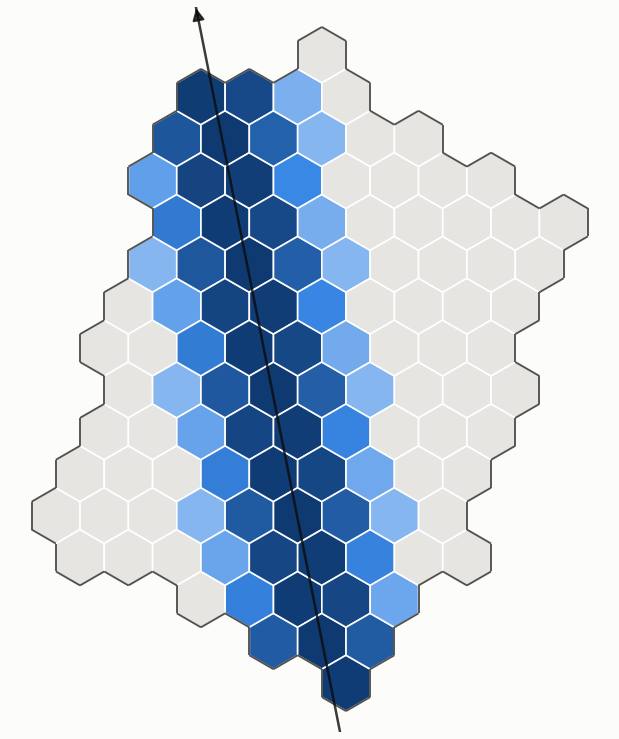
\includegraphics[width=0.48\columnwidth]{concept-river.png}\hfill
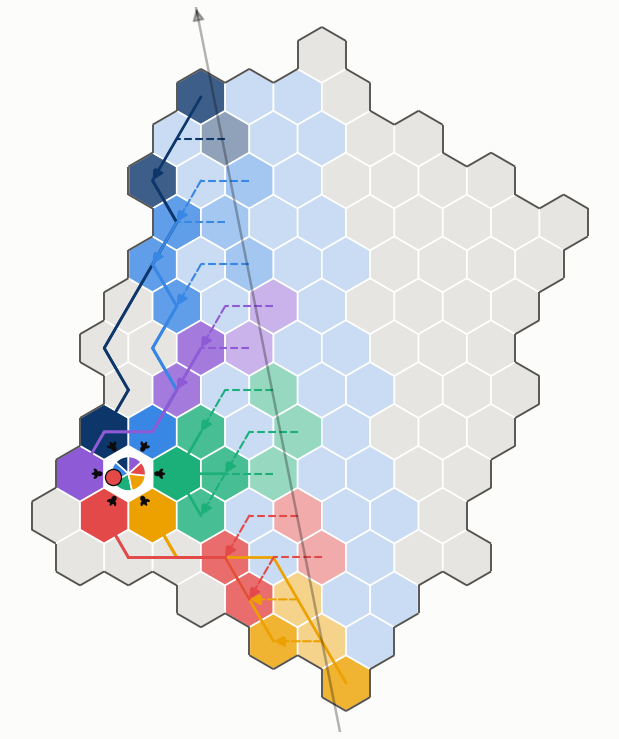
\includegraphics[width=0.48\columnwidth]{concept-circle.png}
\caption{River roles on a cluster with a straight path. Left: \spine{} cells under the path (dark blue), the River band
(lighter towards its edge) and the Banks at the edge. Right: the Ring around a critical cell (red dot); each helper
fetches one group of consecutive segments from the Banks and hands it over in one hop.}\label{fig:roles}
\end{figure}

\begin{algorithm}[t]\caption{River planning at the BS (before take-off)}\label{alg:plan}
\begin{algorithmic}[1]\footnotesize
\REQUIRE path $\gamma$, cluster cells, critical cells $K_c$, range regime
\STATE \spine{} $\leftarrow$ cells crossed by $\gamma$; $\mathrm{Seg}(a)\leftarrow\{s:\gamma(s\Tp)\in a\}$
\FORALL{$a\in$ \spine{}, side $\pm$}
\STATE walk along the local normal of $\gamma$ up to $\omega$ (inner side of a bend: up to the radius of curvature);
$\mathrm{Bank}_\pm(a)\leftarrow$ last cell reached; store the cell path
\ENDFOR
\FORALL{$k\in K_c$}
\STATE $D_k\leftarrow$ the copy of the query emitted nearest to $k$
\STATE helpers $\leftarrow$ 2--12 cells of rings 1--2 around $k$, sized to the predicted lack of $k$
\STATE split \spine{}$\cap D_k$ into consecutive groups; helper $j$ fetches group $j$ from the nearer Banks along
precomputed cell paths
\ENDFOR
\STATE send all tables to the CHs with the flight plan
\end{algorithmic}
\end{algorithm}

\begin{algorithm}[t]\caption{River execution (after the UAV leaves the cluster)}\label{alg:exec}
\begin{algorithmic}[1]\footnotesize
\STATE \textbf{Gather:} in cells with a role, nodes send their CL what the role needs
\STATE \textbf{Bank fill:} a Bank sends a ``have'' manifest of $\mathrm{Seg}(a)$; \spine{} cell $a$ returns what is missing
\STATE \textbf{Repair:} a \spine{} cell completes its segment from adjacent cells; if still incomplete, \textsc{Takeover}
(Algorithm~\ref{alg:takeover})
\STATE \textbf{Ring fill:} helper $j$ requests its group from its Banks
\REPEAT
\STATE \textbf{Final hop:} $k$ sends each helper its lack within the group; the helper forwards packets as they arrive
\UNTIL{$k$ holds $D_k$ (coded: $N'$ packets); a cell idle for 20\,s asks again}
\STATE match and report via the CH
\end{algorithmic}
\end{algorithm}

All steps overlap packet by packet. Requests are ``have'' manifests that fit in one frame. Because the roles depend only
on $\gamma$, River needs no route discovery and no content discovery. With a fountain-coded broadcast the plan is
unchanged except that manifests become counts. The same routes, reversed, let a critical cell pull event crops from the
legacy cameras attached to it; this direction is described in the conference version and not evaluated here.

\textbf{Why it is robust to the range.} River sources data only from the \spine, which receives its own segment whatever
the A2G range. When the range is large it has less to move; when it is small it still completes, whereas schemes that
rely on what a cell hears directly do not.

\subsection{A single-radio lower bound and River's distance from it}
Let $L_k$ be the number of packets of $D_k$ that no node of critical cell $k$ received (its \emph{lack}).
\begin{proposition}\label{prop:radio}
For any ground schedule, critical cell $k$ cannot complete earlier than $\tau_{\min}L_k$ after the UAV has left: every
missing packet must be received by the single radio of its CL over the medium of cell $k$.
\end{proposition}
On 225 critical-cell completions at $R_{50}=99$\,m (experiment of Section~\ref{sec:ground}), cells lack 3744 packets on
average, so the bound is 18\,s. River completes them in 103\,s on average, a median factor 5.1 above the bound; planned
direct pulling is at 5.0 and Deluge at 7.3--7.6 (Fig.~\ref{fig:ground}). A regression over 812 critical cells of 12 runs
(three maps, four regimes) explains where the factor comes from:
\begin{equation}
\widehat T_{\mathrm{River}}(k)=0.71+2.29\,\mathrm{hops}_k+1.97\,\tfrac{L_k}{1000}+4.26\,\tfrac{L_{c(k)}}{1000}\ \text{(s)},\label{eq:surrogate}
\end{equation}
where $\mathrm{hops}_k$ is the cell distance from $k$ to the \spine{} and $L_{c(k)}$ the total lack of the critical cells
of its cluster. A cell's own packets cost about $\tau_f$ each, as the bound predicts, but the packets of the \emph{other}
critical cells of the cluster cost another 4.3\,ms each: the flows share \spine{} cells, Banks and gateways, and each
flow carries its own copy of the same segments. Leave-one-map-out, \eqref{eq:surrogate} has a mean absolute error of
22.8\,s ($R^2=0.60$). Closing the gap to Proposition~\ref{prop:radio} requires forwarding each segment once along a
shared tree instead of once per critical cell; we leave this to future work (Section~\ref{sec:discussion}).

\begin{figure}[t]\centering
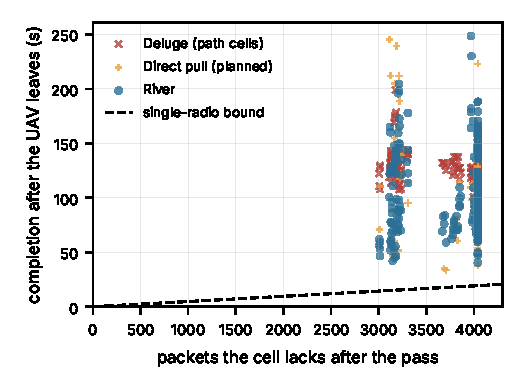
\includegraphics[width=0.82\columnwidth]{ground-lb.pdf}
\caption{Completion time of each critical cell after the UAV has left, against the packets it lacks, for three ground
transports on the same passes (8 clusters, $R_{50}=99$\,m, five network realisations), and the single-radio bound of
Proposition~\ref{prop:radio}.}\label{fig:ground}
\end{figure}

\subsection{Takeover: keeping the plan valid under trajectory error}\label{sec:takeover}
The plan assigns $\mathrm{Seg}(a)$ to \spine{} cell $a$ from the \emph{planned} path. If wind pushes the UAV sideways by
about one reception range, the packets of $\mathrm{Seg}(a)$ are heard by cells that are not adjacent to $a$; the repair
from adjacent cells then fails, and every Bank, Ring and critical cell downstream waits. Takeover restores the segment
without abandoning the plan (Algorithm~\ref{alg:takeover}). Every packet header carries its sequence number and the
position at which it was emitted, so a cell knows which segment a packet belongs to and how far the UAV was from the
planned path.

\begin{algorithm}[t]\caption{\textsc{Takeover} at \spine{} cell $a$ and at a holder cell $c$}\label{alg:takeover}
\begin{algorithmic}[1]\footnotesize
\STATE \textbf{at $a$}, after gathering and the repair from adjacent cells:
\STATE $M\leftarrow\mathrm{Seg}(a)$ minus what $a$ and its adjacent cells hold; \textbf{if} $M=\emptyset$ \textbf{stop}
\STATE $\hat e\leftarrow$ largest distance to the planned path among the emission positions in the headers that $a$ or an
adjacent cell received around $\mathrm{Seg}(a)$
\STATE $h\leftarrow\lceil\hat e/(\sqrt3R_{\mathrm c})\rceil+1$ \ ($h_{\max}$ if no header was received)
\STATE flood \textsc{Query}$(a,M)$ over the cell tree rooted at $a$, $h$ cell hops deep
\STATE \textbf{at $c$}, on \textsc{Query}$(a,M)$: \textbf{if} $c$ holds packets of $M$ that were emitted above $c$ or an
adjacent cell \textbf{then} return them along the reverse path
\STATE \textbf{at $a$}: store the packets; \textbf{if} $M$ is still not covered and $h<h_{\max}$ \textbf{then}
$h\leftarrow h+1$ and flood the new ring
\STATE River continues unchanged: \spine{} $\to$ Bank $\to$ Ring $\to$ critical cell
\end{algorithmic}
\end{algorithm}

Takeover is a repair with respect to an existing plan, not run-time content discovery: when the flight follows the plan
no frame is sent. The following characterises when it is triggered.
\begin{proposition}[Activation]\label{prop:act}
Let $x_s$ be the actual emission position of packet $s$ and $\mathcal N(a)$ the cells adjacent to $a$. Under
independent receptions, takeover is triggered at \spine{} cell $a$ with probability
\begin{equation}
P_{\mathrm{act}}(a)=1-\!\!\prod_{s\in\mathrm{Seg}(a)}\Bigl[1-\!\!\prod_{u\in U_a\cup U_{\mathcal N(a)}}\!\!\bigl(1-p(\lVert x_s-u\rVert)\bigr)\Bigr].\label{eq:act}
\end{equation}
\end{proposition}
On the 840 \spine{} cells of the wind experiment of Section~\ref{sec:wind}, \eqref{eq:act} predicts 2.0, 18.2 and 51.7
activations for deviations of standard deviation 50, 100 and 200\,m; the ns-3 passes show 3, 17 and 48
(Fig.~\ref{fig:act}). Activation rises smoothly with the cross-track deviation $e$ over the segment rather than at a hard
threshold, from below 0.1 for $e<200$\,m to 0.36 at 200--300\,m and 0.92 beyond. Activations at small $e$ are packets that \emph{no} cell
heard, which only a retransmission can repair; activations in which another cell holds the packets---the ones takeover
serves---appear only for $e\ge100$\,m, about one reception range, and never at 50\,m.

\textbf{Query radius.} In the 51 activations with holders, the farthest holder is at most
$\lceil e/(\sqrt3R_{\mathrm c})\rceil+1$ cell hops from $a$, with equality in 9 of them; this is the rule of line~4.
We state it as an empirical rule: a proof needs an assumption on where holders lie, because in the worst direction of
the hexagonal grid one hop covers only $1.5R_{\mathrm c}$. Table~\ref{tab:radius} evaluates the rule offline on the real
pass bitmaps. A fixed radius of 3 hops, as in our ns-3 implementation, reaches all holders at 100\,m but misses two cells
at 200\,m; the adaptive rule with the deviation estimated from received headers reaches 9/9 and 41/42 at its first
attempt while flooding fewer cells than the smallest fixed radius that reaches everything (19.8 against 20.8 cells at
100\,m, 29.7 against 34.0 at 200\,m); the expanding step of line~7 covers the remaining cell.

\begin{figure}[t]\centering
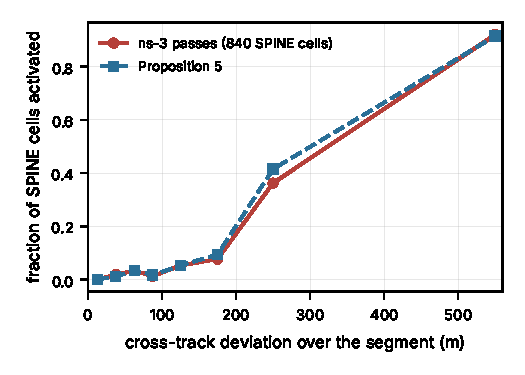
\includegraphics[width=0.8\columnwidth]{propb-activation.pdf}
\caption{Fraction of \spine{} cells in which takeover is triggered versus the cross-track deviation over their segment:
ns-3 passes and Proposition~\ref{prop:act}.}\label{fig:act}
\end{figure}

\begin{table}[t]\centering
\caption{Query radius of takeover, evaluated on the ns-3 wind passes ($R_{50}=99$\,m): activations whose farthest holder
lies inside the flood, and cells flooded per query.}\label{tab:radius}
\footnotesize
\begin{tabular}{lcccc}\toprule
 & \multicolumn{2}{c}{$\sigma=100$\,m (9 activ.)} & \multicolumn{2}{c}{$\sigma=200$\,m (42 activ.)}\\
Rule & reached & cells & reached & cells\\\midrule
fixed 2 hops & 6 & 11.1 & 34 & 13.2\\
fixed 3 hops & 9 & 20.8 & 40 & 23.2\\
fixed 4 hops & 9 & 30.6 & 42 & 34.0\\
adaptive, estimated $\hat e$ & 9 & 19.8 & 41 & 29.7\\
adaptive, true $e$ & 9 & 19.8 & 42 & 29.2\\\bottomrule
\end{tabular}
\end{table}

\section{Flight Design for the Ground Transport}\label{sec:flight}
The path decides the reception map, so it is designed for River rather than for coverage.

\subsection{The delivery constraint}
Every cluster must be offered one complete copy of the query on its own cells, i.e., $Q\Tp=40.4$\,s of emission inside
the cluster. If the path through a cluster is shorter than $Q\Delta$, the UAV slows down, and if the minimum speed is not
enough it adds a loop of radius 63.7\,m at the CH. We call this adjustment \textsc{Fit}. Its consequence shapes the
design: a short path flown slowly costs the same in-cluster time as a long chord flown fast. What a planner can change
is therefore the transit between clusters, the visiting order, and how close the path comes to the cells that matter.

\subsection{\chord}
\chord{} flies one straight line through each cluster, through the CH, at the bearing of the longest in-cluster run; a
long chord gives a long \spine{} and hence many sources for River. The visiting order and directions minimise the mean
time at which critical cells are left behind, $\sum_c n_c\,t^{\mathrm{leave}}_c$ with $n_c$ the number of critical cells
of cluster $c$, by dynamic programming over (cluster, direction) with Dubins transits. The path is the same in every
A2G regime.

\subsection{\lmtour}
\lmtour{} replaces the longest chord by a path that is short and well placed (Algorithm~\ref{alg:lmtour}).

\emph{Step 1: tour through the cluster heads.} For each cluster and each of six bearings, a straight leg through the CH
is cut to its run over the cluster and passed through \textsc{Fit}; its cost is its delivery-feasible duration. The
legs, directions and order minimising $\sum_cW_c\,t^{\mathrm{leave}}_c$, with $W_c$ the total weight of the critical
cells of cluster $c$, are found by dynamic programming with Dubins transits. This is a DTSPN through discs of radius
$\xi$ around the CHs with
\begin{equation}
\xi=\min\bigl(\omega,\ \rho,\ R_{50}\bigr),
\end{equation}
so that a landmark within $\xi$ lies in the River band, the path can still turn there, and the landmark hears the UAV
directly; $\xi=255$, 255, 199 and 99\,m in the four regimes.

\emph{Step 2: bending towards landmarks.} Within each cluster the leg is bent, by smooth bumps of curvature at most
$1/\rho$ with the CH pinned, into the disc $B(k,\xi)$ of a critical cell $k$ whenever this lowers
\begin{equation}
\begin{aligned}
J_c=&\sum_{k\in K_c}w_k\,\mathrm{ready}_k+\Bigl(\sum_{k\in K_c}w_k\Bigr)t^{\mathrm{in}}_c\\
&+\theta\,W^{\mathrm{after}}_c\bigl(t^{\mathrm{in}}_c+\mathrm{dur}_c+t^{\mathrm{out}}_c\bigr),
\end{aligned}\label{eq:J}
\end{equation}
where $\mathrm{ready}_k=\min\{\mathrm{own}_k,\ \mathrm{dur}_c+\widehat T_{\mathrm{River}}(k)\}$ is the earlier of the cell
decoding by itself along the pass and River completing it, $\mathrm{dur}_c$ is the pass duration after \textsc{Fit},
$t^{\mathrm{in}}_c,t^{\mathrm{out}}_c$ are the Dubins transits to the neighbouring passes and $W^{\mathrm{after}}_c$ is
the weight of the clusters flown later. $\widehat T_{\mathrm{River}}$ is the surrogate \eqref{eq:surrogate}, evaluated on
the River plan of the candidate path. Bending stops when no candidate lowers $J_c$.

\begin{algorithm}[t]\caption{\lmtour}\label{alg:lmtour}
\begin{algorithmic}[1]\footnotesize
\REQUIRE clusters with CH and critical cells, weights $w$, $\xi$, $\theta$
\FORALL{cluster $c$, bearing $b\in\{0^\circ,30^\circ,\dots,150^\circ\}$}
\STATE $\ell_{c,b}\leftarrow$ line through $\mathrm{CH}_c$ at bearing $b$, cut to its run over $c$; cost
$\leftarrow$ duration of \textsc{Fit}$(\ell_{c,b})$
\ENDFOR
\STATE (legs, directions, order) $\leftarrow\argmin\sum_cW_c\,t^{\mathrm{leave}}_c$ with Dubins transits
\FORALL{cluster $c$}
\STATE $\mathit{cur}\leftarrow$ leg of $c$; $\mathit{pulls}\leftarrow\emptyset$
\REPEAT
\FORALL{$k\in K_c\setminus\mathit{pulls}$ with $w_k\ge w_{\min}$ farther than $\xi$ from $\mathit{cur}$}
\STATE $\gamma_k\leftarrow$ leg bent into $B(k',\xi)$ for $k'\in\mathit{pulls}\cup\{k\}$; keep it if it crosses $c$ once
\STATE evaluate $J_c(\gamma_k)$: \textsc{Fit}, River plan, surrogate \eqref{eq:surrogate}
\ENDFOR
\STATE $k^\star\leftarrow\argmin_kJ_c(\gamma_k)$; \textbf{if} $J_c(\gamma_{k^\star})<J_c(\mathit{cur})$ \textbf{then}
$\mathit{pulls}\leftarrow\mathit{pulls}\cup\{k^\star\}$, $\mathit{cur}\leftarrow\gamma_{k^\star}$
\UNTIL{no improvement}
\ENDFOR
\RETURN the passes and their River plans
\end{algorithmic}
\end{algorithm}

\textbf{Surrogate.} Running ns-3 for every candidate is infeasible, so the BS uses \eqref{eq:surrogate}, fitted on the
completion times of 812 critical cells in ns-3. Its three features are computable before take-off from the path, the
deployment and the channel regime; the lack predicted by the reception model matches the lack observed in ns-3 (mean
2200 against 2183 packets). At mission level the predicted difference between \lmtour{} and \chord{} is within 10\,s of
the one later measured in ns-3 ($-38$, $-93$, $-89$, $-90$\,s predicted against $-38$, $-83$, $-84$, $-90$\,s measured on the
8-cluster map), which is what the planner needs: a ranking of paths.

\textbf{What the two steps contribute.} Because of the delivery constraint, the tour of Step~1 already yields most of the
gain over \chord: the in-cluster time stays near 40\,s while the transits shrink. Bending adds 7--22\,s on the
8-cluster map and saturates after one or two pulls per cluster, since pulling the path towards a cell changes that
cell's hop count and part of its lack but hardly the total lack of the cluster, which dominates \eqref{eq:surrogate}.

\begin{figure*}[t]\centering
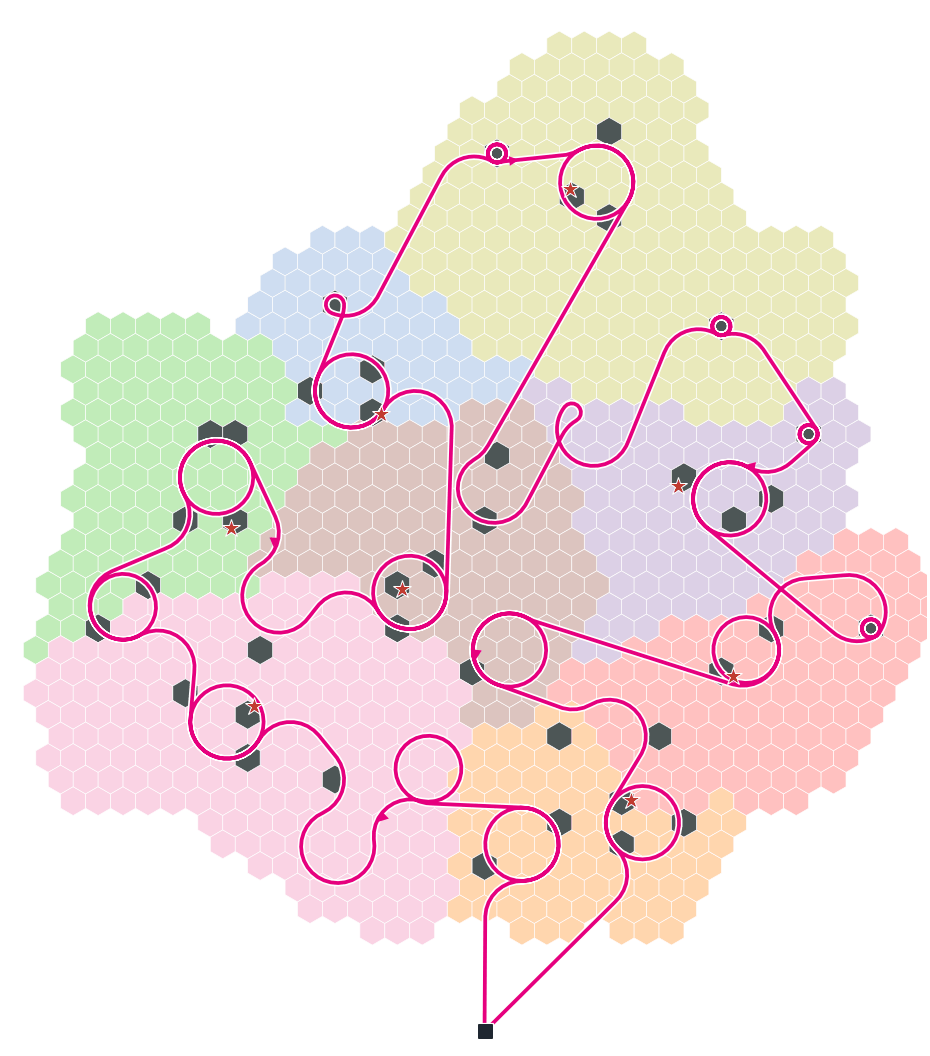
\includegraphics[width=0.21\textwidth]{c4-phase1-k8-s1-r500-fc-dtspn-mono.png}\hfill
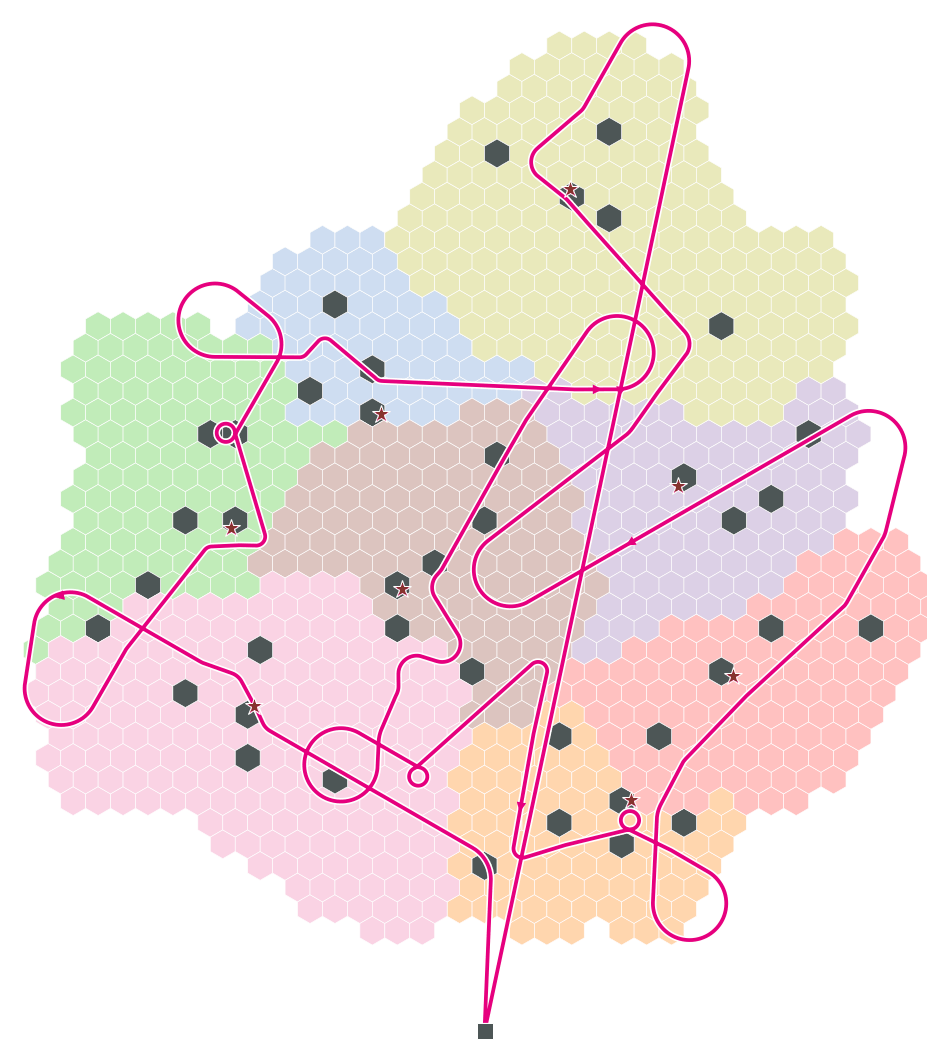
\includegraphics[width=0.21\textwidth]{c4-phase1-k8-s1-r500-dtspn-river-mono.png}\hfill
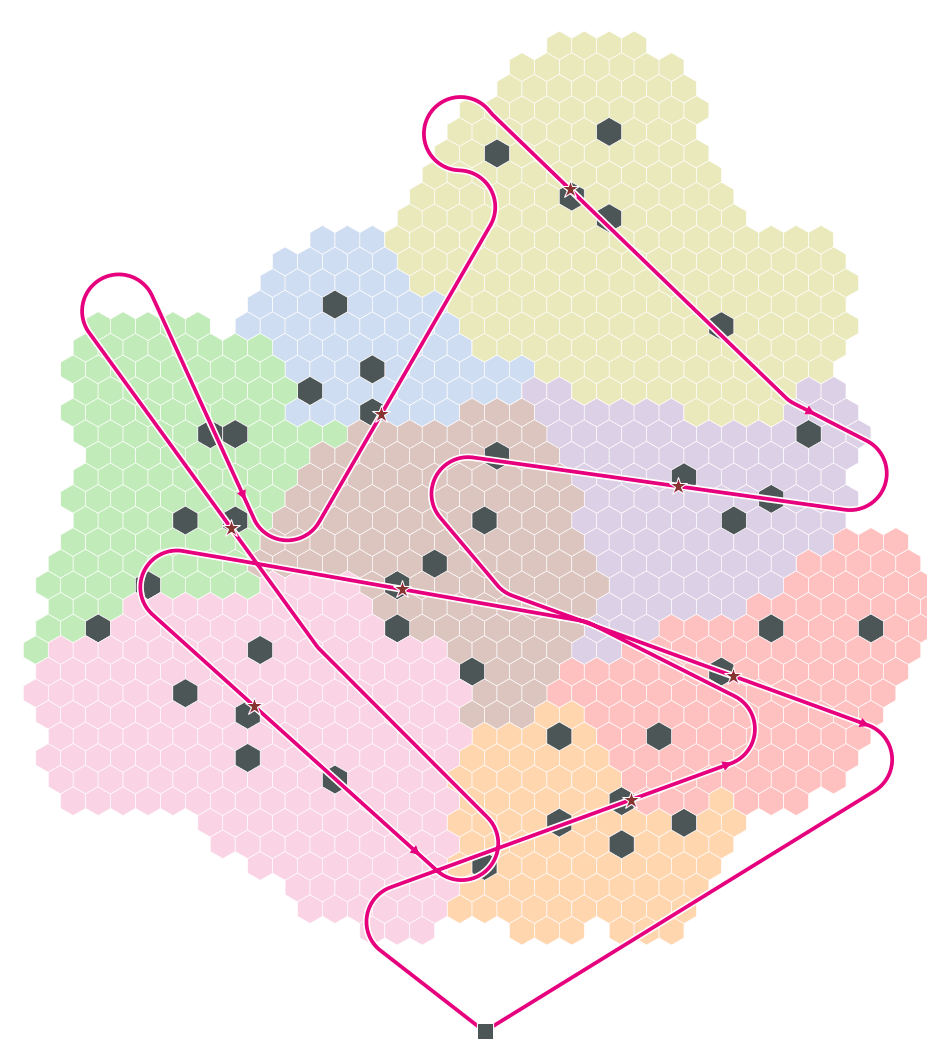
\includegraphics[width=0.21\textwidth]{c4-phase1-k8-s1-r500-chord-mono.png}\hfill
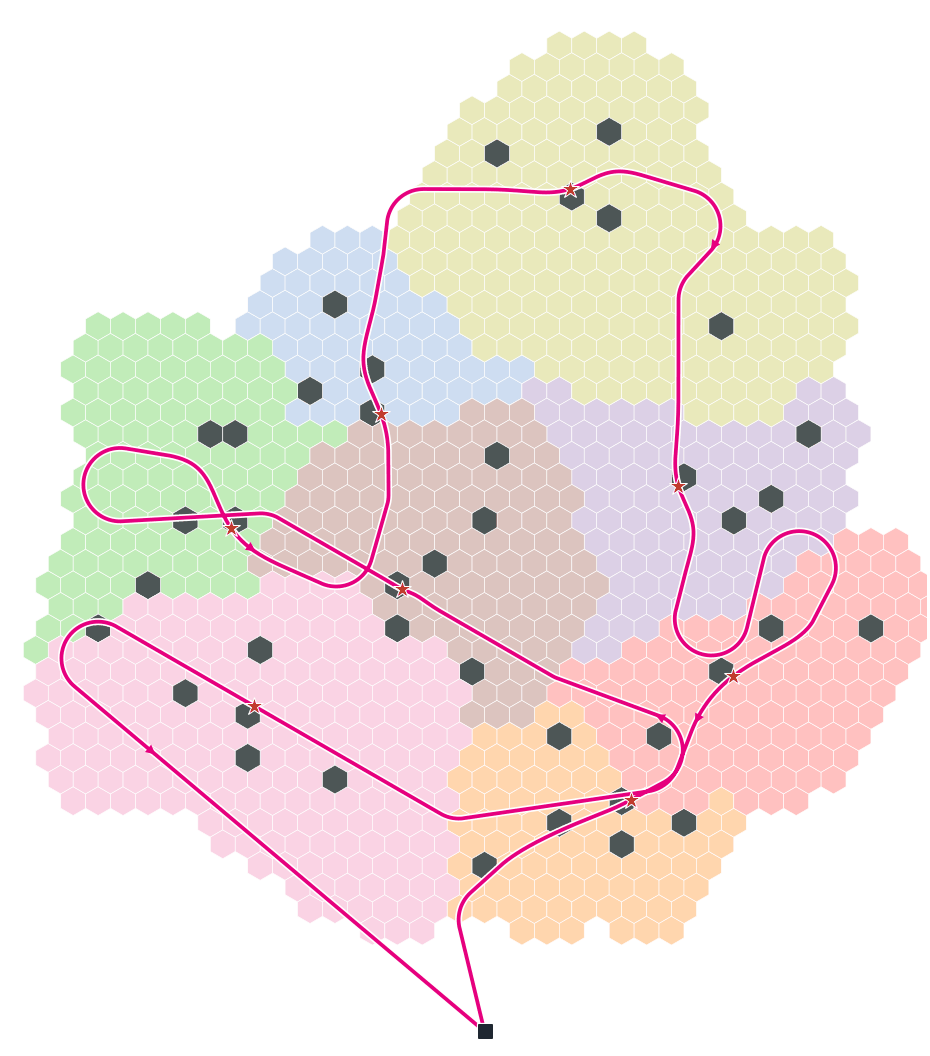
\includegraphics[width=0.21\textwidth]{c4-phase1-k8-s1-r500-lmtour-mono.png}
\caption{Team-1 paths on the 8-cluster map at $R_{50}=498$\,m. From left: FC+DTSP-N (58.7\,km, 1320\,s, orbits around
groups of critical cells), DTSP-N+River (46.6\,km, 1066\,s, into the disc of every critical cell), \chord{}+River
(38.6\,km, 784\,s) and \lmtour{}+River (30.8\,km, 699\,s; small loops are the \textsc{Fit} loops).}\label{fig:paths}
\end{figure*}

\section{Evaluation}\label{sec:eval}
\subsection{Setup}
\textbf{Simulator.} ns-3.46 with lr-wpan: CSMA/CA, acknowledgements and retransmissions, the channel and radio of
Section~\ref{sec:model}. The network is deployed and organised by one binary, the pass by a second, and the ground
transport by a third; all three are frozen for the campaign.

\textbf{Maps and regimes.} Three maps on a non-convex domain with lakes, with 8, 12 and 15 clusters (capacitated
$k$-medoids, at most 80 cells each) and 45, 66 and 92 critical cells; the smallest has 617 cells and 13\,086 nodes. Four
A2G regimes, $R_{50}=1016$, 498, 199 and 99\,m. Cluster geometry, CHs and critical cells are the same for all schemes.

\textbf{Schemes.} \emph{\lmtour{}+River} and \emph{\chord{}+River} (Section~\ref{sec:flight}), with River's repair
enabled and per-critical-cell windows. \emph{DTSP-N+River}: a Dubins path that enters the disc $B(k,\xi)$ of
\emph{every} critical cell, crossing each cluster once, followed by River; it isolates the value of River from that of
the path. \emph{FC+DTSP-N}: no ground cooperation; the query is coded with an ideal rateless code ($\epsilon=0.05$); Team~1
flies a DTSPN through groups of nearby critical cells (group radius 200, 300 or 400\,m, whichever gives the shortest
plan) and orbits each group until every member has heard enough, in expectation, with a margin of three standard
deviations per image; its receptions follow the channel model rather than a packet-level ns-3 pass. \emph{No broadcast}:
Team~2 alone visits every critical cell with the full reference (a rotary-wing TSP), as an upper reference.

\textbf{Replications.} Ten simulation seeds; a seed fixes the fading of the pass, the shadowing and fading on the ground
and the MAC draws. Each seed is one ns-3 run per cluster and 100 paired draws of the matching layer, shared by all
schemes. The campaign was stopped at 81\,\% of its jobs, so a setting has 6--10 seeds. Confidence intervals are Student-$t$
intervals over per-seed means, because the 100 draws of a seed share one network realisation.

\subsection{Mission time}
Table~\ref{tab:tstar} and Fig.~\ref{fig:tstar} report $T^\star$. \lmtour{}+River is the fastest scheme in every setting.
Against FC+DTSP-N it is 10--14\,\% faster at $R_{50}=1016$\,m, 31--38\,\% at 498\,m and 59--72\,\% at 199 and 99\,m; the
gap widens as the range shrinks because the fountain-coded baseline must orbit until every cell has heard enough by
itself. From the widest to the narrowest range, $T^\star$ of \lmtour{}+River grows by 30--39\,\%, that of FC+DTSP-N by a
factor 3.3--4.3. The whole single-pass architecture is 3.5--5.8 times faster than having no broadcast phase.

\begin{table*}[t]\centering
\caption{Mean mission time $T^\star$ (s) on the maps with 8 / 12 / 15 clusters; ns-3, 6--10 seeds of 100 paired draws
each. Half-widths of the 95\,\% confidence intervals are 41--231\,s (per setting in the supplementary data).}\label{tab:tstar}
\footnotesize
\begin{tabular}{lcccc}\toprule
Scheme & $R_{50}=1016$\,m & 498\,m & 199\,m & 99\,m\\\midrule
No broadcast (rotary TSP) & 2809 / 4227 / 5242 & 2809 / 4227 / 5242 & 2809 / 4227 / 5242 & 2852 / 4194 / 5242 \\
FC + DTSP-N & 689 / 914 / 1062 & 1063 / 1545 / 1895 & 1911 / 2715 / 3710 & 2268 / 3368 / 4523 \\
DTSP-N + River & 751 / 887 / 1084 & 917 / 1187 / 1454 & 975 / 1340 / 1666 & 1055 / 1371 / 1658 \\
\chord{} + River & 658 / 814 / 939 & 778 / 1101 / 1200 & 847 / 1161 / 1321 & 872 / 1165 / 1335 \\
\lmtour{} + River & 618 / 803 / 911 & 730 / 981 / 1171 & 791 / 1053 / 1237 & 806 / 1054 / 1262 \\
\bottomrule\end{tabular}
\end{table*}

\begin{figure*}[t]\centering
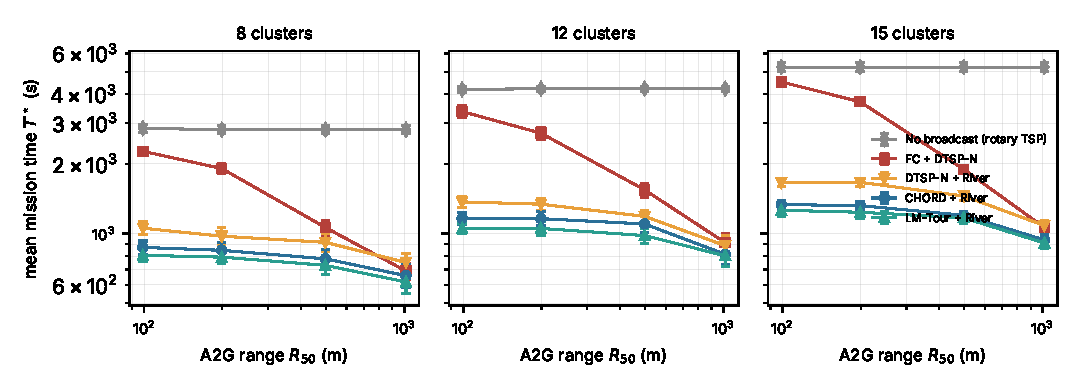
\includegraphics[width=0.86\textwidth]{tstar-c4.pdf}
\caption{Mean mission time versus A2G range, with 95\,\% confidence intervals over seeds.}\label{fig:tstar}
\end{figure*}

\textbf{Value of River.} DTSP-N+River against FC+DTSP-N isolates the ground transport: it is 14--23\,\% faster at 498\,m
and 49--63\,\% at 199 and 99\,m. Over open land it is not faster ($-3$ to $+9$\,\%): its zigzag path is longer than the
baseline's and River has little to move. River is a mechanism for short range.

\textbf{Choosing the path for the ground.} \lmtour{} is 10--26\,\% faster than DTSP-N+River although both use River and
the same tour solver. Flying close to every critical cell does not pay: on the 15-cluster map at 199\,m, \lmtour{} brings
only 36 of 92 critical cells within $\xi$ of the path (\chord{} 42, DTSP-N+River all 92) and is the fastest.
Against \chord{}, \lmtour{} is 1--11\,\% faster with a path 14--28\,\% shorter; the difference is significant (the
95\,\% interval of the paired per-seed difference excludes zero) in 10 of 12 settings.

\subsection{Anatomy of phase~1}
Table~\ref{tab:phase1} separates the flight from the ground. The flight of the River schemes is nearly independent of
the range, because the delivery constraint fixes the in-cluster time: on the 15-cluster map at 199\,m a pass takes 43.3\,s
with \chord{} (2099\,m at 48\,m/s), 40.5\,s with \lmtour{} (1560\,m at 38.5\,m/s) and 62.4\,s with DTSP-N+River (2438\,m),
whose path through every disc exceeds one copy of the query. FC+DTSP-N has the shortest tour over open land (30.5\,km on
the 8-cluster map) and by far the longest at short range (113\,km), where it orbits. The mean time at which critical
cells are ready, from take-off, is 58--106\,s earlier with \lmtour{} than with \chord{}; the difference in $T^\star$ is
smaller because phase~2 dilutes it.

\begin{table}[t]\centering
\caption{Phase~1 on the maps with 8 / 12 / 15 clusters: Team-1 flight time and mean time, from take-off, at which
critical cells are complete (s).}\label{tab:phase1}
\setlength{\tabcolsep}{2.5pt}\footnotesize
\begin{tabular}{llcc}\toprule
 & $R_{50}$ & flight & mean completion\\\midrule
FC+DTSP-N & 1016 & 669 / 913 / 1134 & \\
 & 498 & 1320 / 2011 / 2563 & \\
 & 199 & 2687 / 4016 / 5567 & \\
 & 99 & 3305 / 5078 / 6808 & \\\midrule
DTSP-N+River & 1016 & 1066 / 1553 / 2007 & 504 / 713 / 934\\
 & 99 & 1170 / 1589 / 2105 & 630 / 860 / 1066\\\midrule
\chord{}+River & 1016 & 784 / 1292 / 1437 & 360 / 566 / 701\\
 & 498 & 784 / 1292 / 1437 & 401 / 607 / 745\\
 & 199 & 784 / 1292 / 1437 & 438 / 643 / 777\\
 & 99 & 784 / 1292 / 1437 & 453 / 660 / 796\\\midrule
\lmtour{}+River & 1016 & 698 / 1085 / 1394 & 302 / 473 / 612\\
 & 498 & 699 / 1085 / 1308 & 338 / 508 / 654\\
 & 199 & 697 / 1083 / 1293 & 374 / 544 / 692\\
 & 99 & 708 / 1082 / 1291 & 389 / 554 / 705\\\bottomrule
\end{tabular}
\end{table}

\subsection{Ground transport: planning versus discovery}\label{sec:ground}
On the \chord{} passes of the 8-cluster map at $R_{50}=99$\,m, with five network realisations, we replace River by two
alternatives. \emph{Deluge}: advertise--request dissemination with Trickle timers ($I_{\min}=1$\,s, $I_{\max}=64$\,s,
$k=1$) and 64-packet pages aligned to image and segment boundaries, either on the cells of River's plan or only on the
\spine, the critical cells and the cells between them; radios are always on and there is no low-power listening.
\emph{Planned direct pull}: every critical cell asks each \spine{} cell for what it lacks along the shortest cell path,
with the same repair as River (two realisations).

\begin{table}[t]\centering
\caption{Ground transport on the same passes (8 clusters, $R_{50}=99$\,m), per cluster. Deluge: $\Delta$ is River minus
Deluge, mean $\pm$ 95\,\% CI over 40 (seed, cluster) pairs.}\label{tab:ground}
\setlength{\tabcolsep}{2pt}\scriptsize
\begin{tabular}{lccc}\toprule
 & River & Deluge, plan cells & Deluge, path cells\\\midrule
critical cells complete & 225/225 & 225/225 & 225/225\\
last critical cell ready (s) & 117 & 156 ($-39\pm12$) & 149 ($-32\pm12$)\\
frames sent ($10^3$) & 957 & 2344 ($-1386\pm139$) & 1786 ($-829\pm147$)\\
hop transmissions ($10^3$) & 432 & 1069 & 815\\
\quad of which control & 1.5 & 54.5 & 41.2\\
radio energy, always on (J) & 11\,059 & 14\,943 & 11\,001\\
radio energy, sched.\ sleep (J) & 1693 & 14\,943 & 11\,001\\
hottest node, sched.\ sleep (J) & 19.0 & 28.7 & 27.0\\
$T^\star$ (s) & 863 & 906 ($-43\pm8$) & 899 ($-36\pm7$)\\\bottomrule
\end{tabular}
\end{table}

Table~\ref{tab:ground} shows that all three deliver everything; River readies the last critical cell of a cluster
32--39\,s earlier, sends 1.9--2.5 times fewer frames, and lowers $T^\star$ by 36--43\,s. Two points qualify these numbers.

\emph{The saving is not control overhead.} Control frames are about 5\,\% of Deluge's transmissions. Deluge moves
1.7--2.2 times more \emph{data}, because every cell in scope must complete every page before it can advertise it, and it
is slower because each hop waits for a Trickle timer and a complete page. The energy advantage (6.5--8.8 times, CC2420
model \todo{datasheet citation}) comes from River's nodes sleeping after their last scheduled transmission while Deluge
must keep listening; with all radios always on the energies are within a factor 1.0--1.35. The sleeping figure is an
ex-post bound, optimistic in that it ignores wake-ups for repair requests.

\emph{The saving comes from planning.} Planned direct pull, which also knows in advance who holds what, matches River at
this range: 121 against 119\,s for the last critical cell and 873 against 870\,s for $T^\star$ on the two realisations
where both ran, with 11\,\% fewer frames. River's structure (Banks and Rings) pays off when paths to several critical
cells contend: on a single 80-cell cluster with four critical cells over open land it completes the last one 26\,\%
earlier with 12\,\% fewer frames than direct pulling, and with 4, 7 and 16 critical cells on a 91-cell cluster it uses
20--22\,\% fewer frames in 20 of 20 paired passes. What beats discovery is therefore the plan itself; the particular
shape of the plan matters in dense clusters.

\subsection{Trajectory error and takeover}\label{sec:wind}
The BS plans River on the intended path; the ns-3 pass flies a perturbed one. Lateral and along-track deviations are
white noise smoothed by a Gaussian kernel of 10\,s, with stationary standard deviation $\sigma$ laterally and $\sigma/2$
along the track; packet $s$ is still emitted at $s\Tp$, only its position changes. Flight tests of small fixed-wing
aircraft report cross-track errors of a few metres \cite{park2007,nelson2007}, so $\sigma=50$\,m is already
conservative; $\sigma=100$\,m is of the order of the overshoot of a turn planned in still air under strong wind
\cite{techy2009}, and equals the reception range of this regime. We use the 8-cluster map at $R_{50}=99$\,m, the
narrowest range, with three realisations.

\begin{table}[t]\centering
\caption{River under trajectory error (8 clusters, $R_{50}=99$\,m), without and with takeover: critical cells complete,
and readiness (per cluster, time of the last critical cell after the UAV leaves, mean over clusters; 900\,s if
incomplete).}\label{tab:wind}
\setlength{\tabcolsep}{2.5pt}\scriptsize
\begin{tabular}{cccc}\toprule
$\sigma$ (m) & seed & complete, without $\to$ with & readiness (s): on-plan / without / with\\\midrule
50 & 1 & 45 $\to$ 45 & 126 / 115 / 113\\
50 & 2 & 45 $\to$ 45 & 112 / 113 / 113\\
50 & 3 & 45 $\to$ 45 & 115 / 115 / 114\\
100 & 1 & 33 $\to$ 45 & 126 / 305 / 117\\
100 & 2 & 40 $\to$ 45 & 112 / 214 / 112\\
100 & 3 & 33 $\to$ 45 & 115 / 313 / 118\\\bottomrule
\end{tabular}
\end{table}

At $\sigma=50$\,m nothing breaks and takeover sends no frame (Table~\ref{tab:wind}). At $\sigma=100$\,m, River without
takeover completes only 106 of 135 critical cells and $T^\star$ rises by 294\,s; with takeover all 135 complete, readiness
returns to 112--118\,s (nominal 112--126\,s), and the mean $T^\star$ equals the on-plan value within run-to-run noise
($+0.2\pm121$\,s; per seed $-20$, $-35$, $+56$\,s, the same spread as at 50\,m where takeover is idle). In these runs the
holders are found from the real reception bitmaps without simulating the query. In a second implementation the \spine{}
cell floods a query over three cell hops with real control frames after the repair from adjacent cells has finished;
the results are unchanged: 135 of 135 complete, readiness 112--118\,s, total frames within $\pm3$\,\%, $T^\star$ minus
nominal $-22\pm184$\,s. (In a single realisation at $\sigma=200$\,m, which exceeds 1\,g of lateral acceleration at
times, River alone completes 3 of 45 critical cells and River with takeover 45 of 45.) The adaptive radius of
Algorithm~\ref{alg:takeover} is evaluated offline in Table~\ref{tab:radius}.

\subsection{Where to place the AI nodes}\label{sec:aicells}
So far $K$ was fixed by score outliers. Here $K$ is chosen, with the legacy cameras of Section~\ref{sec:model} sending,
before any incident, one record per passer-by to the nearest AI node of their cluster: a frame (40\,kB), a person crop
(10\,kB) or a feature vector (512-d INT8 plus 16\,B, 528\,B). Records travel only inside the mesh, from a camera to its
AI node; the BS still receives scores only. The background load uses the per-cell model fitted on the River trace (1.5 frames per
packet at the end cells, 1.7 in transit, 1 per gateway pair, 6.5\,ms per frame); every medium may be busy at most 10\,\% of
the time and 30\,\% of the nodes are cameras, each seen by $\rho$ people per hour.

\textbf{Which record.} On the 8-cluster map, with 8 to 128 AI cells placed by $k$-medoids, the largest $\rho$ under the
budget is 0.2--1.9 for frames, 0.7--7.7 for crops and 13--145 for vectors; the busiest medium is the cell of the AI node
itself. Frames and crops are therefore infeasible at any urban flow, and only vectors are kept. The 45 critical cells of
the outlier rule carry at most 18 people/h and lie up to 8 cells from some assigned node.

\textbf{Choosing $K$.} For each $\rho$ we take the fewest AI cells per cluster that keep the busiest medium under the
budget with every node at most $H=5$ cell hops from its AI cell (a capacitated facility location), placed by local search
on the River surrogate. Table~\ref{tab:aicells} lists the result: fewer than the outlier rule up to $\rho=50$, more above.
Fig.~\ref{fig:k9surr} checks the surrogate in ns-3 (both $R_{50}=199$ and 99\,m, one seed): up to 70 AI cells the
measured end of phase~1 is within 41\,s of the model and the order of the sets is kept, except that at 199\,m 69 AI
cells finish 12\,s after the outlier set instead of 41\,s before. With 161 AI cells (20 per cluster, outside the range
the surrogate was fitted on) the model fails: in one cluster ns-3 spreads from 75 to more than 900\,s, and phase~1 ends
at 1\,231\,s or later against 906\,s predicted.

\begin{table}[t]\centering\caption{AI cells needed and modelled end of phase~1 (s) at a 10\,\% budget, $R_{50}=99$\,m;
in brackets the ns-3 value (8 clusters, one seed).}\label{tab:aicells}
\begin{tabular}{lccc}\toprule
$\rho$ (people/h) & 8 clusters & 12 clusters & 15 clusters\\\midrule
20 & 24: 661 (687) & 32: 992 & 49: 1162\\
50 & 34: 674 & 52: 1005 & 64: 1168\\
100 & 69: 728 (733) & 98: 1061 & 123: 1235\\
200 & 161: 906 ($\ge$1231) & 220: 1147 & 275: 1362\\
outlier rule & 45: 753 (770) & 66: 1021 & 92: 1232\\\bottomrule
\end{tabular}\end{table}

\begin{figure}[t]\centering
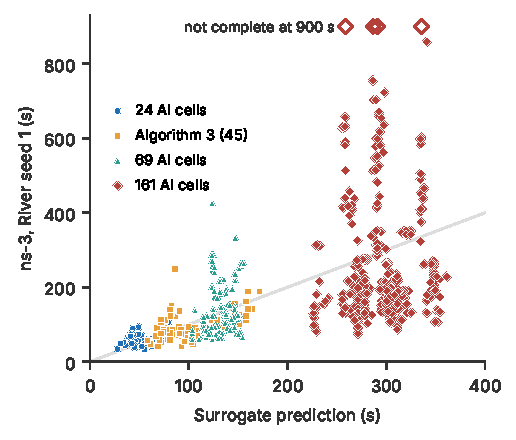
\includegraphics[width=0.9\columnwidth]{k9-surrogate-vs-ns3.pdf}
\caption{End of the query at each AI cell, from the UAV leaving its cluster: River surrogate versus ns-3, for the sets
chosen at $\rho=20$, 100 and 200 and for the outlier rule ($R_{50}=199$ and 99\,m, one seed). Hollow: not complete when
River stops at 900\,s.}\label{fig:k9surr}
\end{figure}

\textbf{Both phases.} Phase~2 follows the model of Section~\ref{sec:model} with verification by re-matching at the AI
node (5\,s to settle and 73\,s to send the full reference). An AI cell indexes $\rho\cdot 2\,\mathrm{h}\cdot 0.3\, n_c$
vectors for its $n_c$ assigned nodes and sets its threshold for a given false-alarm probability; the target passes a
uniformly drawn node. Fig.~\ref{fig:k9time} shows the time until the true AI cell is confirmed at $\rho=20$ (300 paired
draws). With a false-alarm probability of 0.1 per AI cell, the time grows from 823 to 1\,234\,s between 24 and 161 AI
cells, because the AI cells answering YES grow from 2.8 to 16.5. Holding the false alarms of the whole system at 2.4
narrows the gap (823 to 1\,061\,s) without reversing it, and the smaller set then also detects more often (0.63 against
0.58 with one target vector), since its per-cell threshold is lower. A larger index costs little detection: the
threshold grows with the logarithm of the index size.

\begin{figure}[t]\centering
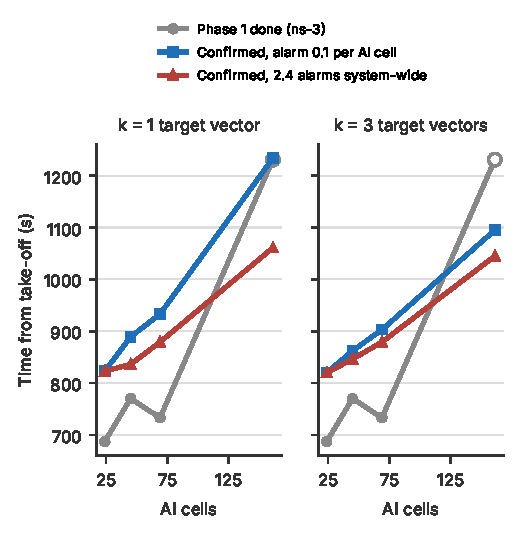
\includegraphics[width=\columnwidth]{k9-time-vs-ai-cells.pdf}
\caption{Time from take-off to the confirmation of the true AI cell versus the number of AI cells, $\rho=20$,
$R_{50}=99$\,m, under the two false-alarm rules; grey: last AI cell holding the query (hollow: lower bound).}\label{fig:k9time}
\end{figure}

\textbf{Sensitivity.} With an AI node in every cell, vectors fit up to $\rho=640$ people/h (1\,275 at a 20\,\% budget),
below a busy commercial street (about 1\,500) and a Manhattan peak (3\,700). All loads and index sizes scale with
$\rho$ times the camera share times the node density, so at 400 and 280 nodes/km$^2$ a set serves about 2.0 and 2.9
times the flow; thinning the nodes cell by cell confirms the scaling within 2\,\% for 24 AI cells but shows up to 23\,\%
more load for 161 AI cells at 280 nodes/km$^2$. The device tier does not change the choice: embedding one crop per
passer-by keeps an ESP32-class camera at most 28\,\% busy, and searching 152\,280 vectors with a 20-image reference takes
at most 5.4\,s at the AI node; only a microcontroller AI node needs external storage for the larger indexes (80\,MB).
\todo{second seed of the ns-3 check; River times at 400 and 280 nodes/km$^2$.}

\subsection{Stability across network realisations}
Differences between schemes that share River are stable across seeds (e.g., \lmtour{} minus DTSP-N+River on the
15-cluster map at 199\,m: $-425$\,s on the first seed, $-429\pm70$\,s on the others). Absolute values are not: with River,
$T^\star$ of other seeds is 56--197\,s above that of the first seed on the 15-cluster map, while a scheme that does not
depend on the mesh varies by $\pm15$\,s. The variation comes from the ns-3 network realisation (fading, MAC), which is
what a multi-seed campaign must capture; no number in this section relies on a single seed unless stated.

\section{Discussion and Limitations}\label{sec:discussion}
\textbf{What the theory does and does not show.} Theorem~\ref{thm:cover} bounds a class of schemes from below; it does
not bound River from above. The comparison in Table~\ref{tab:bounds} therefore pairs a proven limit with measured
flight times. The limit certifies the advantage of cooperation for $R_{50}\le200$\,m on our maps and is silent at longer
range, where the measured advantage (31--38\,\% at 498\,m) rests on the comparison with one concrete baseline. A matching
upper bound for River needs a model of contention on shared cells; the regression \eqref{eq:surrogate} suggests its
form (a term in the cluster's total lack) but is not a proof.

\textbf{Distance from the ground bound.} River completes a critical cell about five times later than the single-radio
bound, and planned direct pulling does no better. The flows towards the critical cells of a cluster carry the same
segments separately. Forwarding each segment once along a tree that branches towards the Rings, or merging the Rings of
nearby critical cells, should remove most of the term in the cluster's total lack; we have not simulated it.

\textbf{Channel model.} Fading is redrawn independently for every packet and nodes fade independently. Our limits do not
need the first assumption, but the simulated reception maps do. Around a ground node the scatterers are local, so the
fading of consecutive packets emitted 0.25--0.5\,m apart is correlated in reality, and shadowing is correlated over tens
of metres \cite{gudmundson1991}, i.e., within a cell; field measurements also show shorter ranges for a moving UAV
\cite{nekrasov2019}. Correlation lowers the cell-level diversity that \eqref{eq:pcell} assumes and should favour
cooperation further, since the \spine{} needs only its own overhead segment; this is to be verified with a correlated
channel calibrated on public measurements \todo{run}.

\textbf{Baselines.} FC+DTSP-N is evaluated with the channel model rather than a packet-level pass, with an ideal code;
both choices favour it. Deluge runs without low-power listening and with a classical parameterisation; modern
synchronous-transmission protocols \cite{doddavenkatappa2013,du2017,ferrari2012} disseminate faster than Deluge on
testbeds but cannot be reproduced in ns-3's lr-wpan model. A duty-cycled Deluge restricted to River's target set and a
channel-switching unicast protocol in the style of \cite{liang2008} are the comparisons still missing \todo{run}.

\textbf{Trajectory error.} The deviation model is synthetic. A model driven by flight dynamics (path-following guidance,
steady wind and turbulence), with along-track error mapped to packet positions, would replace it \todo{run}. Holder
discovery is idealised in the first takeover implementation and uses a fixed radius in the second; the adaptive radius
is evaluated offline only.

\textbf{Scope.} The phase-0 organisation is assumed in place and its cost is not charged to River; since the network
serves many queries, that cost should be amortised and reported per query. One UAV serves the area; a park-scale
deployment calls for several, which turns the tour into a multi-vehicle min--max problem. The event-pull direction and
the matching layer are unchanged from the conference version. Results are for one deployment density and one query size.

\section{Conclusion}
In a single-pass UAV broadcast the flight path is the transmission schedule, so the base station can plan the ground's
cooperation before take-off. We showed that designs without cooperation are limited by a fractional covering number of
the receivers that grows by an order of magnitude as the air-to-ground range shrinks, while a single pass pays the query
airtime once per cluster. River realises the cooperation as a pre-planned transport with a repair that keeps the plan
valid under trajectory error, and \lmtour{} designs the flight for it. In ns-3 the combination is 59--72\,\% faster than
fountain-coded loitering at ranges of 200\,m and below, completes its flight before the proven limit of non-cooperative
delivery, and needs about half the frames of an epidemic protocol. The remaining distance to the single-radio bound on
the ground, a correlated channel and multi-UAV operation are the next steps.

\appendices
\section{Proof of Theorem~\ref{thm:nphard}}\label{app:nphard}
We reduce Exact Cover to the restricted problem: constant speed $v$, turning radius $\rho$, a ground graph without
edges, every critical cell consisting of a single node, and deterministic reception (a node hears a packet if and only
if the horizontal distance to the UAV is at most $\xi$, with $\xi\ge\Delta/2=v\Tp/2$), and $Q=1$.

Papadimitriou \cite{papadimitriou1977} maps an instance of Exact Cover to a set $P$ of $n$ points in the plane and a
number $L$, in polynomial time, such that the shortest Euclidean tour through $P$ has length at most $L$ if the instance
has a solution and at least $L+g$ otherwise, for a constant gap $g>0$ \cite{leny2012}. Savla \emph{et al.}
\cite{savla2008} show that the shortest Dubins tour through any $n$ points exceeds the shortest Euclidean tour by at most
$Cn$, with $C$ proportional to $\rho$. Let $\lambda$ be an integer with $\lambda g>Cn+2n\xi$ and let $\lambda P$ be the
scaled point set. Place one critical cell at every point of $\lambda P$, the BS at one of them, and set
$T=(\lambda L+Cn)/v$.

If Exact Cover has a solution, there is a Dubins tour through all points of $\lambda P$ of length at most
$\lambda L+Cn$. Flown at speed $v$ it ends by time $T$. It passes through the centre of every disc $B(x,\xi)$,
$x\in\lambda P$, hence contains an arc of length at least $2\xi\ge\Delta$ inside the disc, on which at least one packet is
emitted; the single node at $x$ receives it and is complete.

If Exact Cover has no solution, consider any plan under which all cells complete and the UAV returns to the BS. Its
ground track is a closed curve that enters every disc $B(x,\xi)$. Adding to it, at each disc, a detour to the centre and
back of length at most $2\xi$ gives a closed curve through all points of $\lambda P$, of length at least
$\lambda(L+g)$. The track is therefore longer than $\lambda(L+g)-2n\xi>\lambda L+Cn$ and cannot be flown by time $T$.

The construction is polynomial, so the restricted problem, and hence (P0), is NP-hard. \hfill\IEEEQED

\section{Proof of Proposition~\ref{prop:pack}}\label{app:pack}
Let $n\le T/\Tp$ be the number of packets emitted by time $T$, and $n_k$ the number emitted while the UAV is within $D$ of
$c_k$, for $k\in S$. All nodes of cell $k$ lie within $D$ of $c_k$ for the radii considered, so $P_k$ is non-increasing
along rays from $c_k$ outside this disc and $p_k(D)$ is attained on its boundary. As in the proof of
Theorem~\ref{thm:cover}, $(1-\delta)Q\le\mathbb{E}[N_k]\le n_k\bar p_k+n\,p_k(D)$, so
\[
n_k\ \ge\ \bigl((1-\delta)Q-(T/\Tp)\,p_k(D)\bigr)/\bar p_k .
\]
If $T\ge(1-\delta)Q\Tp/\max_{k\in S}p_k(D)$ there is nothing to prove. Otherwise the right-hand side is positive for
every $k\in S$, so $n_k>0$: the UAV enters every disc.
The discs are disjoint, so the UAV spends at least $\Tp\sum_{k\in S}n_k$ inside them. Outside the discs, the track
consists of pieces that join two discs, or a disc and the BS; a piece joining discs $i$ and $j$ is at least
$\lVert c_i-c_j\rVert-2D$ long. Since the track starts at the BS and visits every disc, these pieces
connect all of them, and their total length is at least the weight of a spanning tree under these lengths, which is at
least $W(S)-2D|S|$. Hence $T\ge\Tp\sum_{k\in S}n_k+(W(S)-2D|S|)^+/v_{\max}$; substituting the bound on $n_k$ and
solving for $T$ gives the first term of \eqref{eq:pack}. \hfill\IEEEQED

\begin{thebibliography}{99}\footnotesize
\bibitem{zeng2016mag} Y. Zeng, R. Zhang, and T. J. Lim, ``Wireless communications with unmanned aerial vehicles:
Opportunities and challenges,'' \emph{IEEE Commun. Mag.}, vol. 54, no. 5, pp. 36--42, May 2016.
\bibitem{mozaffari2019} M. Mozaffari, W. Saad, M. Bennis, Y.-H. Nam, and M. Debbah, ``A tutorial on UAVs for wireless
networks: Applications, challenges, and open problems,'' \emph{IEEE Commun. Surveys Tuts.}, vol. 21, no. 3,
pp. 2334--2360, 2019.
\bibitem{shen2020} Y. Shen, Y. Xiong, W. Xia, and S. Soatto, ``Towards backward-compatible representation learning,'' in
\emph{Proc. IEEE/CVF CVPR}, 2020.
\bibitem{zeng2018multicast} Y. Zeng, X. Xu, and R. Zhang, ``Trajectory design for completion time minimization in
UAV-enabled multicasting,'' \emph{IEEE Trans. Wireless Commun.}, vol. 17, no. 4, pp. 2233--2246, Apr. 2018.
\bibitem{luby2002} M. Luby, ``LT codes,'' in \emph{Proc. IEEE FOCS}, 2002, pp. 271--280.
\bibitem{hui2004} J. W. Hui and D. Culler, ``The dynamic behavior of a data dissemination protocol for network
programming at scale,'' in \emph{Proc. ACM SenSys}, 2004, pp. 81--94.
\bibitem{levis2004} P. Levis, N. Patel, D. Culler, and S. Shenker, ``Trickle: A self-regulating algorithm for code
propagation and maintenance in wireless sensor networks,'' in \emph{Proc. USENIX NSDI}, 2004.
\bibitem{wu2018} Q. Wu, Y. Zeng, and R. Zhang, ``Joint trajectory and communication design for multi-UAV enabled wireless
networks,'' \emph{IEEE Trans. Wireless Commun.}, vol. 17, no. 3, pp. 2109--2121, Mar. 2018.
\bibitem{zeng2017energy} Y. Zeng and R. Zhang, ``Energy-efficient UAV communication with trajectory optimization,''
\emph{IEEE Trans. Wireless Commun.}, vol. 16, no. 6, pp. 3747--3760, Jun. 2017.
\bibitem{wang2020d2d} \todo{first author's initials} Wang, R. Zhang, C. Chen \emph{et al.}, ``Graph-based file
dispatching protocol with D2D-enhanced UAV-NOMA communications in large-scale networks,'' \emph{IEEE Internet Things J.},
vol. 7, no. 9, pp. 8615--8630, 2020. \todo{read full text; cited from the abstract only}
\bibitem{miao2020} J. Miao, Q. Liao, and Z. Zhao, ``Joint rate and coverage design for UAV-enabled wireless networks with
underlaid D2D communications,'' in \emph{Proc. IEEE ICCC}, 2020, pp. 815--819.
\bibitem{kulkarni2005} S. S. Kulkarni and L. Wang, ``MNP: Multihop network reprogramming service for sensor networks,''
in \emph{Proc. IEEE ICDCS}, 2005.
\bibitem{liang2008} C.-J. M. Liang, R. Mus\u{a}loiu-E., and A. Terzis, ``Typhoon: A reliable data dissemination
protocol for wireless sensor networks,'' in \emph{Proc. EWSN}, LNCS 4913, 2008, pp. 268--285.
\bibitem{doddavenkatappa2013} M. Doddavenkatappa, M. C. Chan, and B. Leong, ``Splash: Fast data dissemination with
constructive interference in wireless sensor networks,'' in \emph{Proc. USENIX NSDI}, 2013, pp. 269--282.
\bibitem{du2017} W. Du, J. C. Liando, H. Zhang, and M. Li, ``Pando: Fountain-enabled fast data dissemination with
constructive interference,'' \emph{IEEE/ACM Trans. Netw.}, vol. 25, no. 2, 2017.
\bibitem{ferrari2012} F. Ferrari, M. Zimmerling, L. Mottola, and L. Thiele, ``Low-power wireless bus,'' in \emph{Proc.
ACM SenSys}, 2012.
\bibitem{shokrollahi2006} A. Shokrollahi, ``Raptor codes,'' \emph{IEEE Trans. Inf. Theory}, vol. 52, no. 6,
pp. 2551--2567, Jun. 2006.
\bibitem{ho2006} T. Ho \emph{et al.}, ``A random linear network coding approach to multicast,'' \emph{IEEE Trans. Inf.
Theory}, vol. 52, no. 10, pp. 4413--4430, Oct. 2006.
\bibitem{stojanovic2009} I. Stojanovic, Z. Wu, M. Sharif, and D. Starobinski, ``Data dissemination in wireless broadcast
channels: Network coding versus cooperation,'' \emph{IEEE Trans. Wireless Commun.}, vol. 8, no. 4, pp. 1726--1732, 2009.
\bibitem{leny2012} J. Le Ny, E. Feron, and E. Frazzoli, ``On the Dubins traveling salesman problem,'' \emph{IEEE Trans.
Autom. Control}, vol. 57, no. 1, pp. 265--270, Jan. 2012.
\bibitem{isaacs2011} J. T. Isaacs, D. J. Klein, and J. P. Hespanha, ``Algorithms for the traveling salesman problem with
neighborhoods involving a Dubins vehicle,'' in \emph{Proc. American Control Conf.}, 2011, pp. 1704--1709.
\bibitem{noon1993} C. E. Noon and J. C. Bean, ``An efficient transformation of the generalized traveling salesman
problem,'' \emph{INFOR}, vol. 31, no. 1, pp. 39--44, 1993.
\bibitem{obermeyer2009} K. J. Obermeyer, ``Path planning for a UAV performing reconnaissance of static ground targets in
terrain,'' in \emph{Proc. AIAA Guidance, Navigation, and Control Conf.}, 2009.
\bibitem{penicka2019} R. P\v{e}ni\v{c}ka, J. Faigl, M. Saska, and P. V\'a\v{n}a, ``Data collection planning with
non-zero sensing distance for a budget and curvature constrained unmanned aerial vehicle,'' \emph{Auton. Robots},
vol. 43, pp. 1937--1956, 2019.
\bibitem{khawaja2019} W. Khawaja, I. Guvenc, D. W. Matolak, U.-C. Fiebig, and N. Schneckenburger, ``A survey of
air-to-ground propagation channel modeling for unmanned aerial vehicles,'' \emph{IEEE Commun. Surveys Tuts.}, vol. 21,
no. 3, pp. 2361--2391, 2019.
\bibitem{alhourani2014} A. Al-Hourani, S. Kandeepan, and S. Lardner, ``Optimal LAP altitude for maximum coverage,''
\emph{IEEE Wireless Commun. Lett.}, vol. 3, no. 6, pp. 569--572, Dec. 2014.
\bibitem{matolak2017} D. W. Matolak and R. Sun, ``Air--ground channel characterization for unmanned aircraft
systems---Part III: The suburban and near-urban environments,'' \emph{IEEE Trans. Veh. Technol.}, vol. 66, no. 8, 2017.
\bibitem{nekrasov2019} M. Nekrasov, R. Allen, I. Artamonova, and E. Belding, ``Optimizing 802.15.4 outdoor IoT sensor
networks for aerial data collection,'' \emph{Sensors}, vol. 19, no. 16, 3479, 2019.
\bibitem{park2007} S. Park, J. Deyst, and J. P. How, ``Performance and Lyapunov stability of a nonlinear path-following
guidance method,'' \emph{J. Guid. Control Dyn.}, vol. 30, no. 6, pp. 1718--1728, 2007.
\bibitem{nelson2007} D. R. Nelson, D. B. Barber, T. W. McLain, and R. W. Beard, ``Vector field path following for
miniature air vehicles,'' \emph{IEEE Trans. Robot.}, vol. 23, no. 3, pp. 519--529, Jun. 2007.
\bibitem{techy2009} L. Techy and C. A. Woolsey, ``Minimum-time path planning for unmanned aerial vehicles in steady
uniform winds,'' \emph{J. Guid. Control Dyn.}, vol. 32, no. 6, pp. 1736--1746, 2009.
\bibitem{schroff2015} F. Schroff, D. Kalenichenko, and J. Philbin, ``FaceNet: A unified embedding for face recognition
and clustering,'' in \emph{Proc. IEEE CVPR}, 2015.
\bibitem{deng2019} J. Deng, J. Guo, N. Xue, and S. Zafeiriou, ``ArcFace: Additive angular margin loss for deep face
recognition,'' in \emph{Proc. IEEE/CVF CVPR}, 2019.
\bibitem{ye2022} M. Ye \emph{et al.}, ``Deep learning for person re-identification: A survey and outlook,'' \emph{IEEE
Trans. Pattern Anal. Mach. Intell.}, vol. 44, no. 6, pp. 2872--2893, 2022.
\bibitem{tr38901} 3GPP, ``Study on channel model for frequencies from 0.5 to 100 GHz,'' TR 38.901.
\bibitem{etsi220} ETSI EN 300 220-2 V3.2.1, 2018.
\bibitem{papadimitriou1977} C. H. Papadimitriou, ``The Euclidean travelling salesman problem is NP-complete,''
\emph{Theor. Comput. Sci.}, vol. 4, no. 3, pp. 237--244, 1977.
\bibitem{savla2008} K. Savla, E. Frazzoli, and F. Bullo, ``Traveling salesperson problems for the Dubins vehicle,''
\emph{IEEE Trans. Autom. Control}, vol. 53, no. 6, pp. 1378--1391, Jul. 2008.
\bibitem{gudmundson1991} M. Gudmundson, ``Correlation model for shadow fading in mobile radio systems,'' \emph{Electron.
Lett.}, vol. 27, no. 23, pp. 2145--2146, 1991.
\end{thebibliography}


\end{document}
